\chapter{Resultados e discussões}
\label{chapter:Resultados}

\section{Parâmetros de entrada} \label{section:parametrosdeentrada}
Ao analisar o banco de dados disponibilizado por \citeonline{Neves2019}, obteve-se as distribuições de ocorrência em relação aos parâmetros observados (Figura \ref{fig:db_hist}).

\begin{figure}[h]
	\caption{Distribuições de ocorrência} %of{figure}
	\label{fig:db_hist}
	\centering
	\begin{minipage}{.33\textwidth}
		\centering
		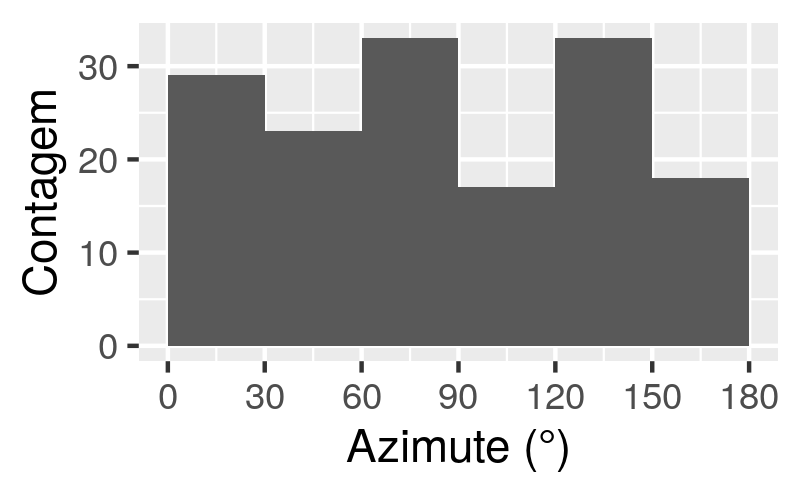
\includegraphics[width=\linewidth]{img/hist_azimute.png}
	\end{minipage}%
	\begin{minipage}{.33\textwidth}
		\centering
		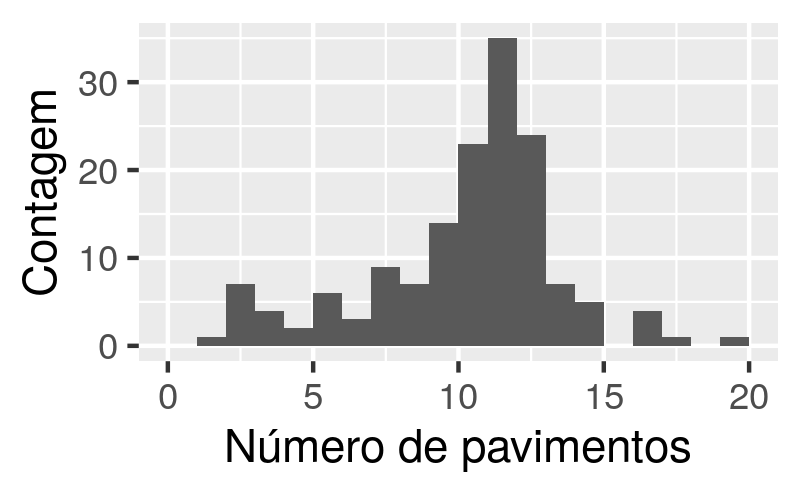
\includegraphics[width=\linewidth]{img/hist_numero_pavimentos.png}
	\end{minipage}%
	\begin{minipage}{.33\textwidth}
		\centering
		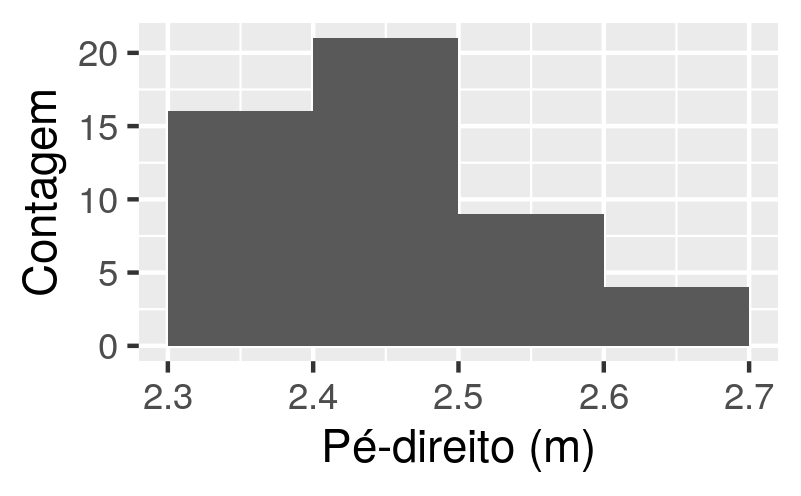
\includegraphics[width=\linewidth]{img/hist_pe_direito.png}
	\end{minipage}
	\centering
	\begin{minipage}{.33\textwidth}
		\centering
		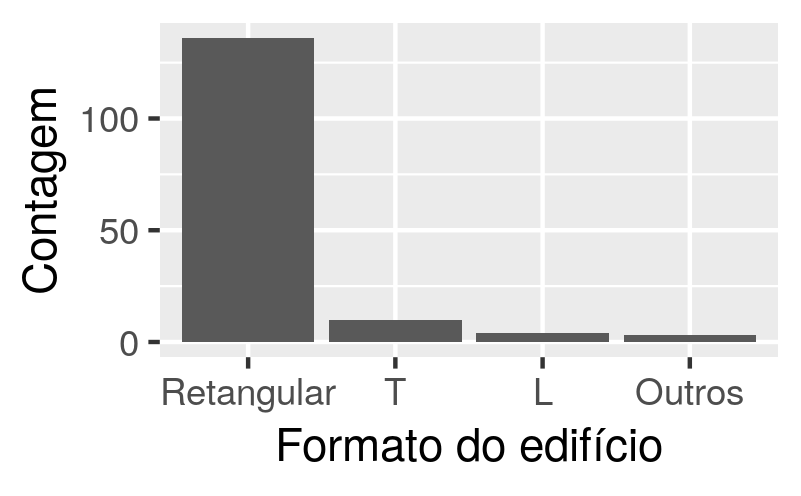
\includegraphics[width=\linewidth]{img/hist_formato.png}
	\end{minipage}%
	\begin{minipage}{.33\textwidth}
		\centering
		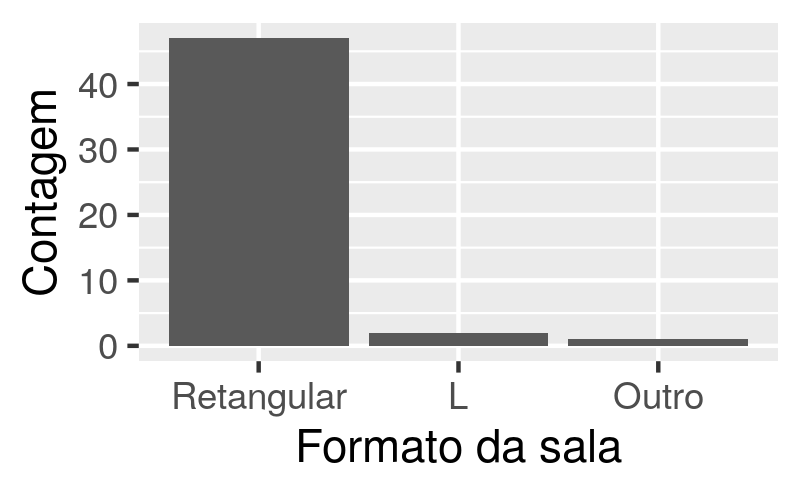
\includegraphics[width=\linewidth]{img/hist_formato_sala.png}
	\end{minipage}%
	\begin{minipage}{.33\textwidth}
		\centering
		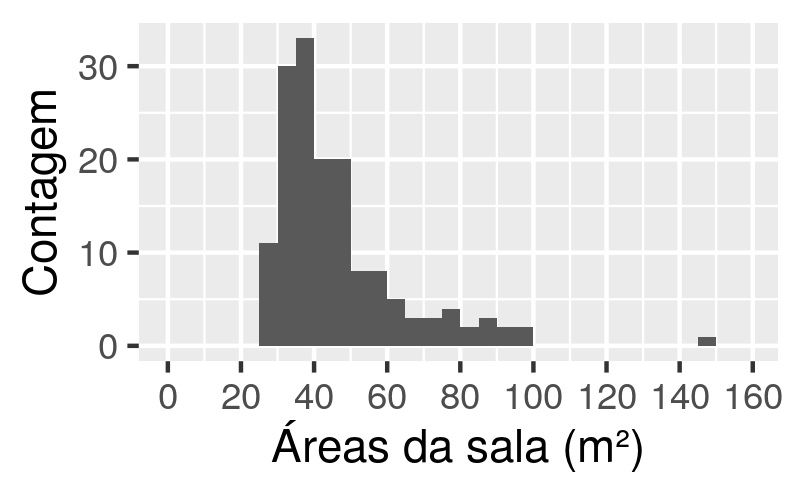
\includegraphics[width=\linewidth]{img/hist_area_zonas.png}
	\end{minipage}
	\centering
	\begin{minipage}{.33\textwidth}
		\centering
		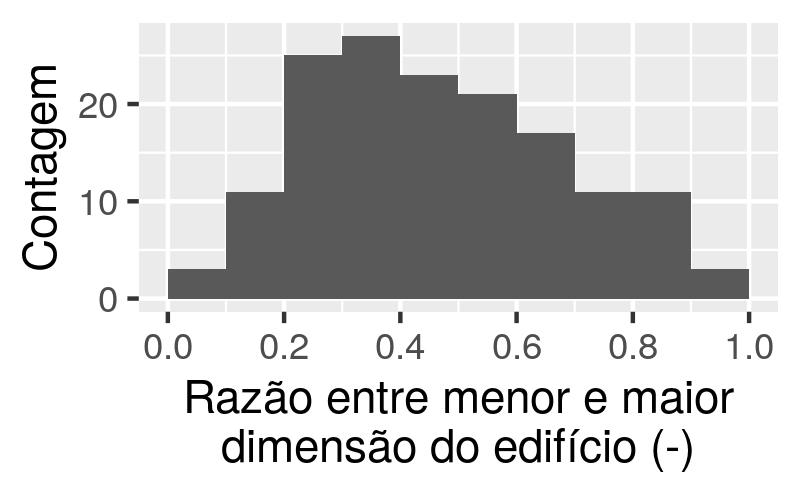
\includegraphics[width=\linewidth]{img/hist_ratio_edificio.png}
	\end{minipage}%
	\begin{minipage}{.33\textwidth}
		\centering
		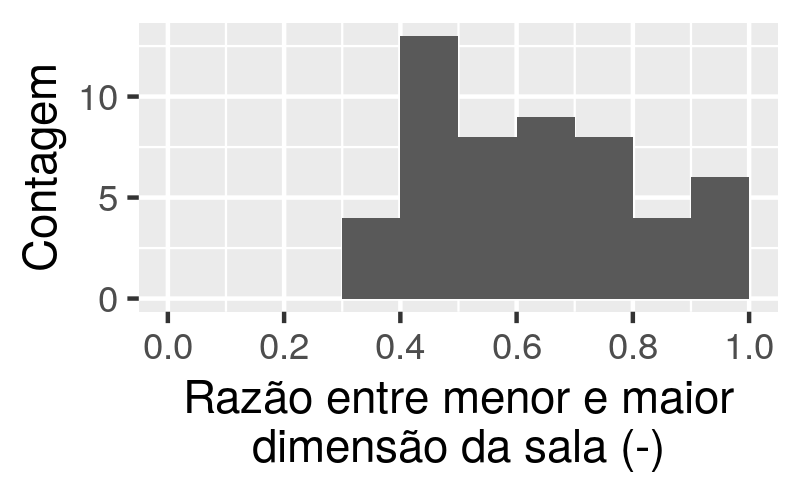
\includegraphics[width=\linewidth]{img/hist_ratio_sala.png}
	\end{minipage}%
	%\end{figure}
	%\begin{figure}
	%	\ContinuedFloat
	%	\caption[]{\textit{Continuação}} % {figure}
	%	\centering	
	\begin{minipage}{.33\textwidth}
		\centering
		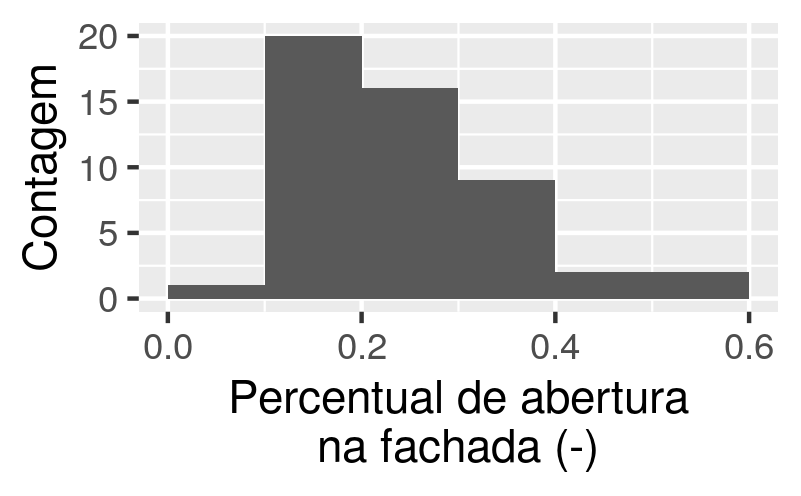
\includegraphics[width=\linewidth]{img/hist_PAF.png}
	\end{minipage}
	\centering
	\begin{minipage}{.33\textwidth}
		\centering
		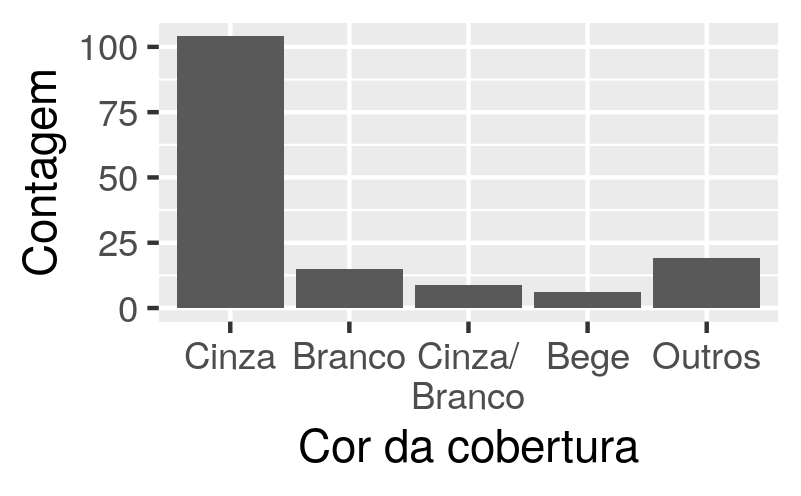
\includegraphics[width=\linewidth]{img/hist_cor_cobertura.png}
	\end{minipage}%
	\begin{minipage}{.33\textwidth}
		\centering
		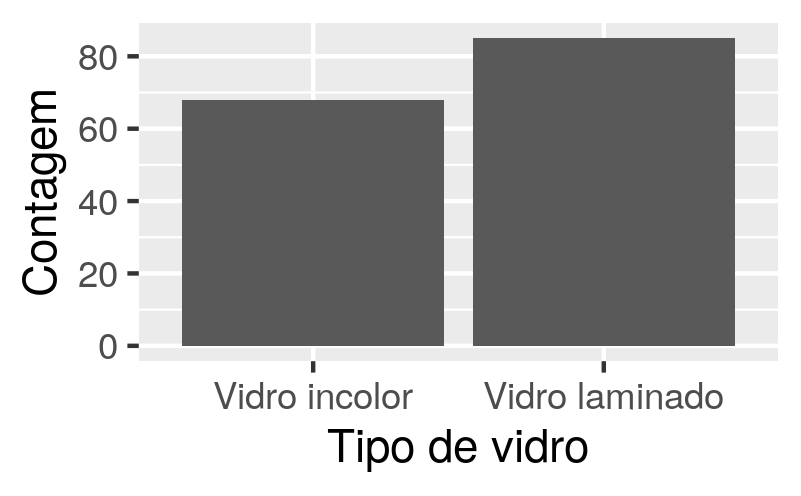
\includegraphics[width=\linewidth]{img/hist_tipo_vidro.png}
	\end{minipage}%
	\begin{minipage}{.33\textwidth}
		\centering
		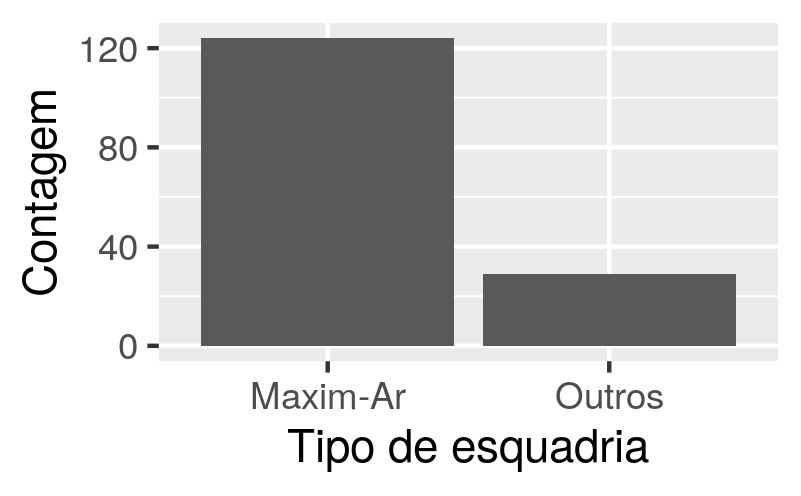
\includegraphics[width=\linewidth]{img/hist_esquadria.png}
	\end{minipage}
	\centering	
	\begin{minipage}{.33\textwidth}
		\centering
		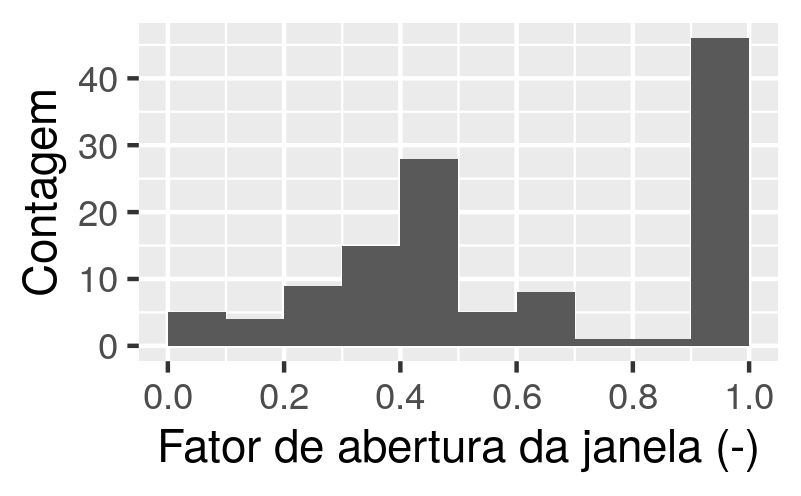
\includegraphics[width=\linewidth]{img/hist_openfac.png}
	\end{minipage}%
	\begin{minipage}{.33\textwidth}
		\centering
		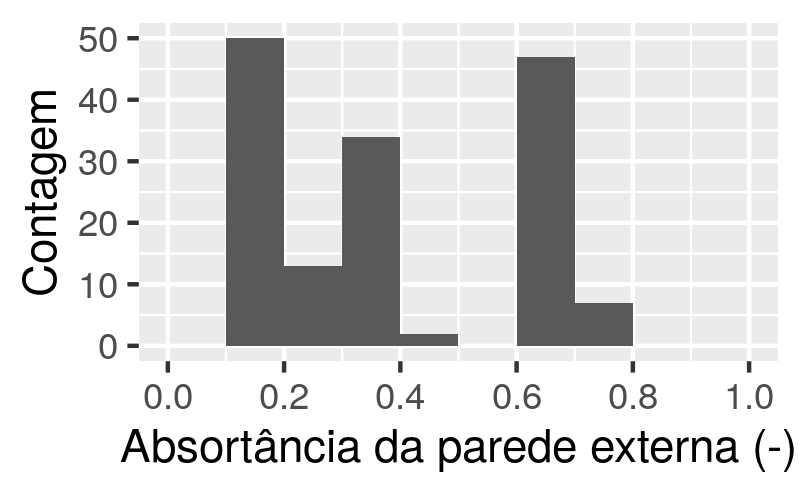
\includegraphics[width=\linewidth]{img/hist_absortancia.png}
	\end{minipage}%
	\begin{minipage}{.33\textwidth}
		\centering
		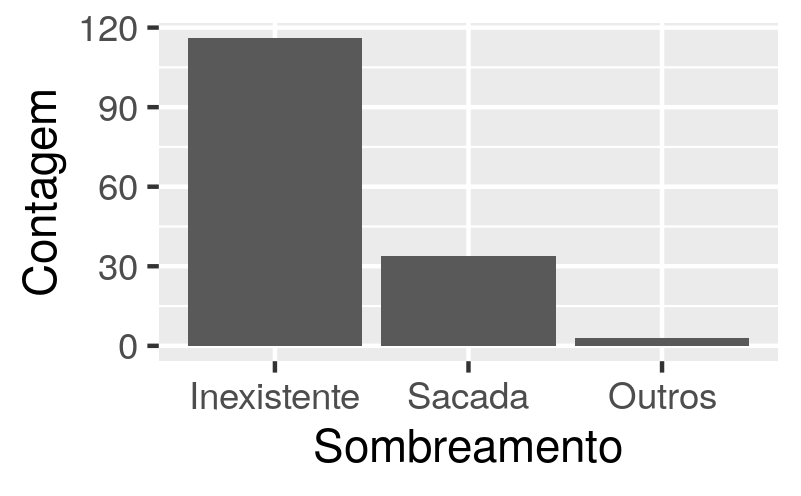
\includegraphics[width=\linewidth]{img/hist_sombreamento.png}
	\end{minipage}
	%	\centering
	\begin{minipage}{.33\textwidth}
		%		\centering
		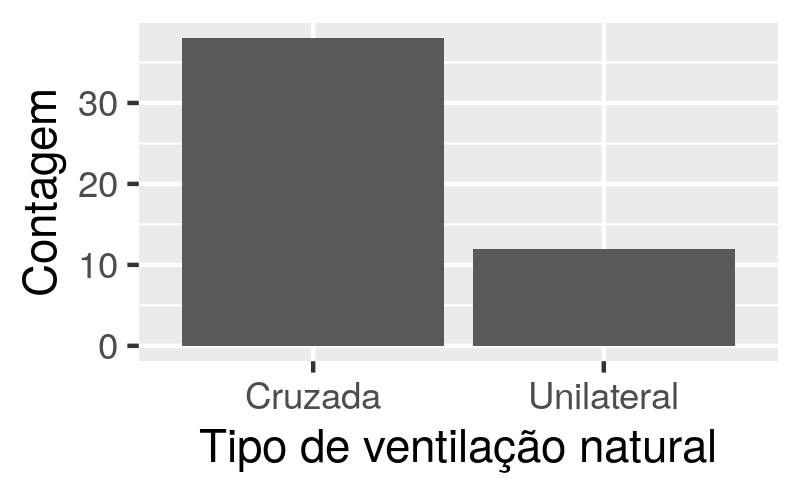
\includegraphics[width=\linewidth]{img/hist_tipo_vn.png}
	\end{minipage}
\end{figure}
%\newpage

O ângulo do azimute é medido em relação ao eixo mais longo das edificações. Observou-se que há ângulos em diversas orientações, indicando que não existe uma orientação predominantemente escolhida para a construção dos edifícios.
O número de pavimentos dos edifícios analisados varia entre 2 e 20 pavimentos, com a maioria das ocorrências em 12 pavimentos.
Tanto os edifícios, quanto as salas existentes no banco de dados apresentam predominantemente formato retangular, a partir do qual considera-se que definir as simulações baseando-se em modelos de edificações retangulares, com salas retangulares, representa adequadamente as tipologias de edifícios encontradas na cidade de São Paulo.
A altura do pé direito não varia significativamente, mas tem a maioria das ocorrências em volta de 2,5 m.
A área das salas de escritório varia entre, aproximadamente, 25 m$^2$ e 160 m$^2$, com a maior ocorrência em valores próximos a 40 m$^2$.
As proporções entre as suas menores e maiores dimensões variam entre, aproximadamente, 0,3 e 1, mas a maior ocorrência está próxima ao valor 0,6.
As proporções entre as menores e maiores dimensões dos pavimentos varia consideravelmente, entre 0,1 e 1.

A absortância das paredes dos edifícios varia entre 0,2 e 0,8, de forma distribuída entre absortâncias baixas, médias e altas. A cor das coberturas é predominantemente cinza. Portanto, foi definido o valor fixo de 0,7 para absortância da cobertura.

Observou-se que esquadrias do tipo maxim-ar são predominantes. Os objetos do \textit{Airflow Network} do programa EnergyPlus não modelam especificamente este tipo de esquadria. Porém, optou-se por considerar as janelas como não pivotantes. Considerar uma janela como horizontalmente pivotante implicaria na consideração de que a abertura acontece simultaneamente na parte de cima e de baixo da janela. No caso da janela maxim-ar, por mais que a abertura aconteça em um eixo horizontal, apenas a parte inferior da janela se abre. 
Os fatores de abertura variam entre zero e um. No entanto, não é aplicável janelas com fatores de abertura igual a zero para edificações com \acrshort{vn}.
O \acrfull{paf} varia entre 0,1 e 0,6 aproximadamente.

O uso de elementos de sombreamento é pouco explorado nas edificações existentes. De qualquer maneira, considerou-se a modelagem de sombreamento horizontal sobre as aberturas da edificação, por considerar o potencial do sombreamento para bloquear a entrada de radiação nas zonas térmicas simuladas. Esse parâmetro foi variado a partir do ângulo de sombreamento formado entre a base da abertura e a proteção solar, localizada no topo da abertura.	
A maioria das salas observadas possuem ventilação cruzada, mas a ventilação unilateral é uma estratégia com ocorrência considerável.

As informações relacionadas ao tipo de vidro não permitem definir valores relacionados ao \acrfull{fs}. Observa-se apenas a ocorrência de vidros laminados e vidro comum incolor. Optou-se por variar o fator solar dos vidros nas simulações para avaliar o impacto deste parâmetro nos resultados de conforto térmico.

%	Os demais parâmetros observados tiveram suas distribuições variando continuamente de acordo com as distribuições obtidas. 
Como as simulações detalhadas foram modeladas como pavimentos da edificação, o parâmetro relacionado ao número de pavimento das edificações foi transformado no parâmetro "altura do pavimento", ou seja, um pavimento localizado em um andar $n$, com um pé-direito de dimensão $h$, foi considerado com uma altura do pavimento igual a $n{\cdot}h$.

A definição dos parâmetros de entrada para o desenvolvimento do metamodelo foi baseada no banco de dados analisados. A Tabela \ref{table:param_def} apresenta os limites mínimos e máximos atribuídos aos diferentes parâmetros contínuos variados nas simulações, assim como os parâmetros variados pela lógica "sim/não". A velocidade do ar foi variada com valores discretos, de acordo com os valores definidos pela \citeonline{ASHRAEStandard552017}, apresentados na Tabela \ref{table:var} do Capítulo \ref{chapter:metodologia}.

\begin{table}[h]
	\centering
	\caption{Limites mínimos e máximos dos parâmetros}
	\label{table:param_def}	
	%	\resizebox{\textwidth}{!}{
	\begin{tabular}{|l |r |}
		\hline
		\textbf{Parâmetro} & \textbf{Valores} \\
		\hline
		Área da sala ($m^2$) & 20 - 100 \\
		\hline
		Razão entre maior e menor da sala ($-$) & 0,4 - 2,5 \\
		\hline
		%		Razão entre maior e menor  & {} \vspace{-7pt}\\
		%		{} & 0,4 - 2,5 \vspace{-7pt}\\ 
		%		da sala ($-$) & {} \\
		%		\hline
		Pé-direito ($m$) & 2,3 - 3,2 \\
		\hline
		Azimute ($^{\circ}$) & 0 - 360 \\
		\hline
		Altura do pavimento ($m$) & 0 - 50 \\
		\hline 
		Absortância da parede ($-$) & 0,2 - 0,8 \\
		\hline 
		Transmitância da parede ($W/m^2K$) & 0,5 - 4,4 \\
		\hline 
		Capacidade térmica da parede ($kJ/m^2K$) & 0,22 - 450,00 \\
		\hline 
		\Acrlong{paf} ($-$) & 0,1 - 0,6 \\
		\hline 
		Fator solar do vidro ($-$) & 0,20 - 0,87 \\
		\hline 
		Sombreamento ($^{\circ}$) & 0 - 80 \\
		\hline 
		Densidade de ocupação ($pessoa/m^2$) & 0,05 - 0,20 \\
		\hline 
		Fator de abertura da janela ($-$) & 0,2 - 1,0 \\
		\hline 
		Razão entre maior e menor dimensão do edifício ($-$) & 0,2 - 1,0 \\
		\hline 
		Cobertura exposta & Sim / Não\\
		\hline 
		Piso exposto & Sim / Não\\
		\hline 
		Ventilação & Cruzada / Unilateral\\
		\hline 
		Velocidade do ar ($m/s$) & 0,0 - 1,2 \\
		\hline 
	\end{tabular}
	%}
	%			\begin{flushleft}
	%				Fonte: \citeauthoronline{INIC} \cite{INIC}, adaptado pelo autor.
	%			\end{flushleft}				
\end{table}

\newpage

\section{Simulações simplificadas}

\subsection*{Cálculo do coeficiente de pressão pelo método analítico}

Ao comparar os valores dos \acrfull{cp} das medições em túnel de vento da \acrfull{tpu} e os valores dos \acrshort{cp} obtidos pelo \acrlong{ma}, obteve-se gráficos de pontos. 
A Figura \ref{fig:cp_diff_scatter}a apresenta a comparação para as 25 proporções geométricas disponibilizadas pela \acrshort{tpu}, para cada fachada, direção do vento, e para cada ponto na fachada.
Como os valores calculados pelo \acrlong{ma} são únicos para cada fachada, e a \acrshort{tpu} oferece valores diferentes para diversos pontos ao longo das fachadas, os pontos no gráfico da Figura \ref{fig:cp_diff_scatter} distribuem-se horizontalmente.
Os pontos vermelhos representam os valores médios da \acrshort{tpu}, para cada geometria, fachada e direção do vento.
%		A Figura \ref{fig:cp_diff_scatter_facade} apresenta a comparação considerando-se os valores médios do \acrshort{cp} para cada fachada. 
É possível observar que a faixa de valores dos \acrshort{cp} disponibilizados pela \acrshort{tpu} é maior do que  faixa de valores calculados pelo \acrlong{ma}. Enquanto o menor valor de \acrshort{cp} disponibilizado pela \acrshort{tpu} é \mbox{-1,40}, e o maior valor é 1,08, pelo \acrlong{ma} o valor mínimo é igual a -0,96 e o máximo é igual a 0,60.

Dentre as geometrias analisadas, a proporção com a maior \gls{rmsecp} entre os valores dos \acrshort{cp} foi igual a 0,42, para a geometria da edificação \textit{highrise} com proporções de largura, profundidade e altura igual a 2:1:2 (Figura \ref{fig:cp_diff_scatter}b).

%\vspace{40pt}

\begin{figure}[h]
	%	\centering
	\caption{Comparação entre os valores de $C_p$ obtidos pelo método analítico e pela base de dados da TPU}
	\begin{minipage}{.5\textwidth}
		%		\centering
		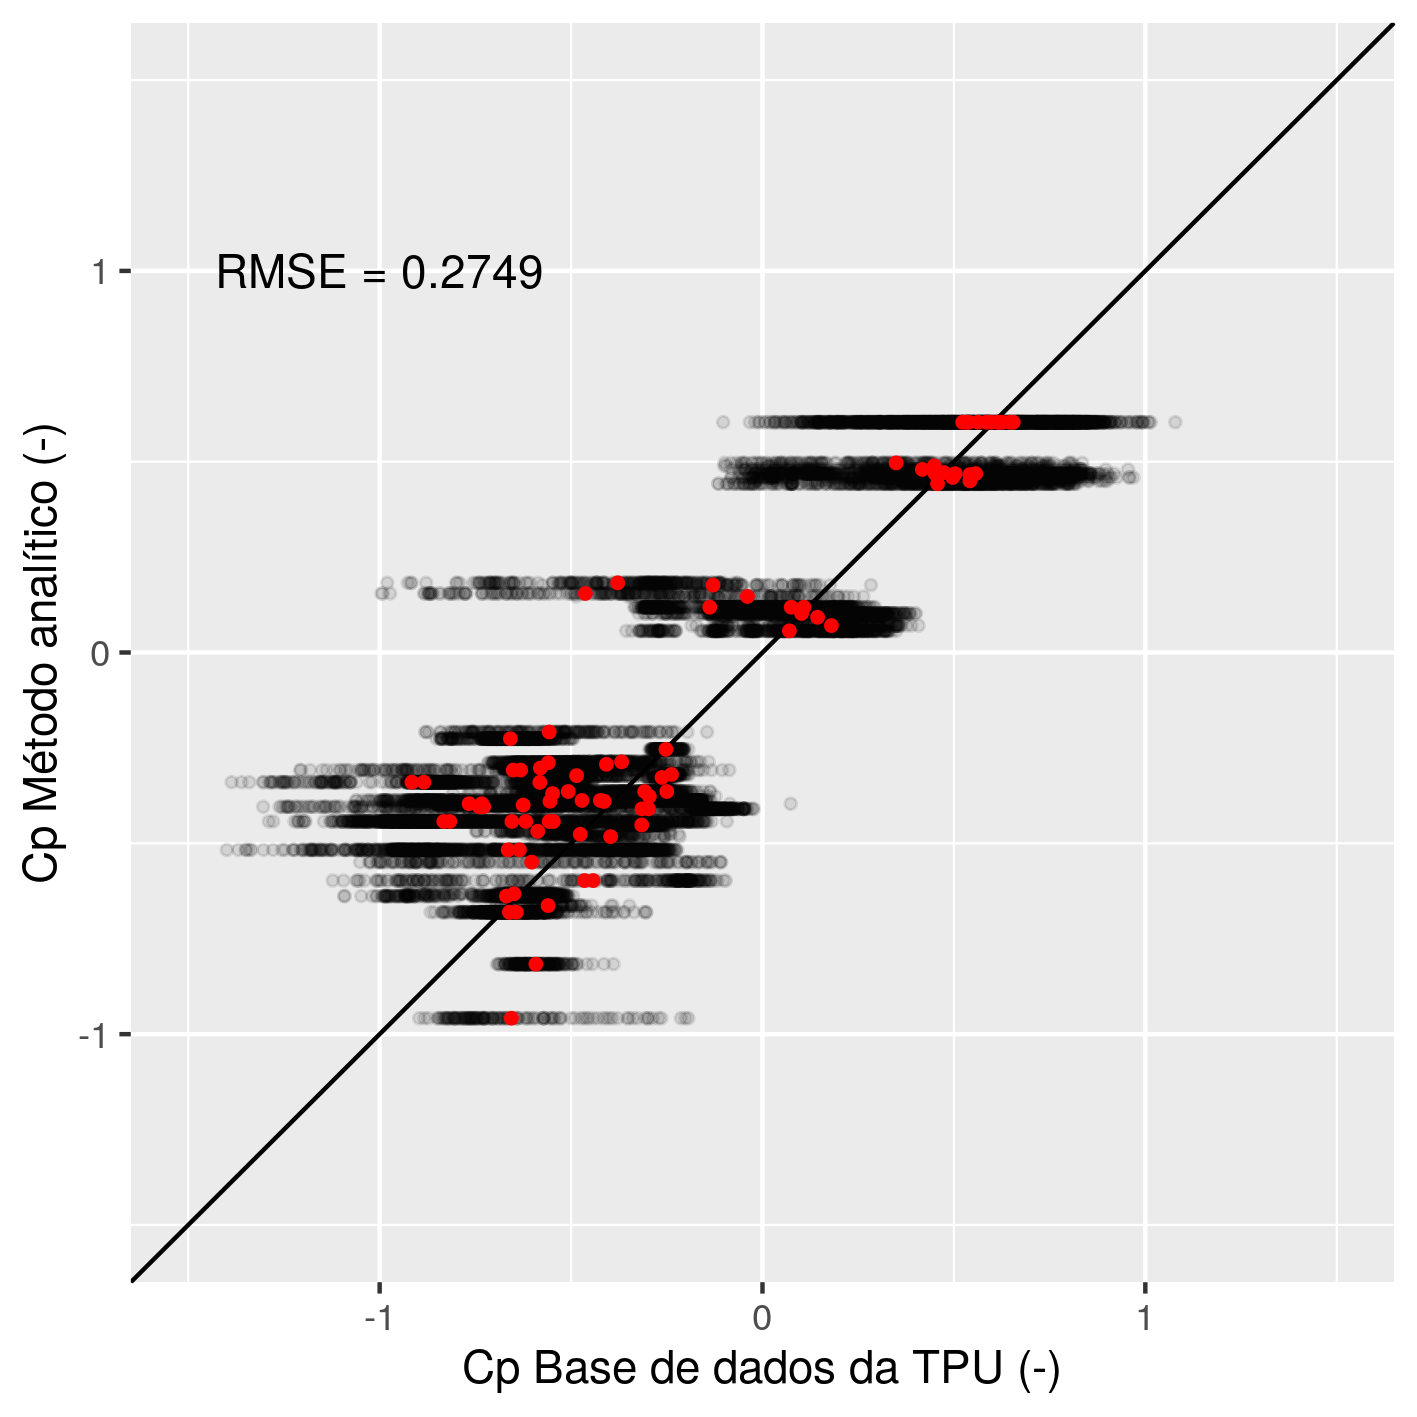
\includegraphics[width=\linewidth]{img/cp_diff_scatter_all.png}
		%		\caption{Comparação entre os valores de \acrshort{cp} das 25 geometrias}
		\begin{center}
			\small{(a) Geometrias de todas as proporções disponíveis}
		\end{center}
	\end{minipage}%
	\begin{minipage}{.5\textwidth}
		%		\centering
		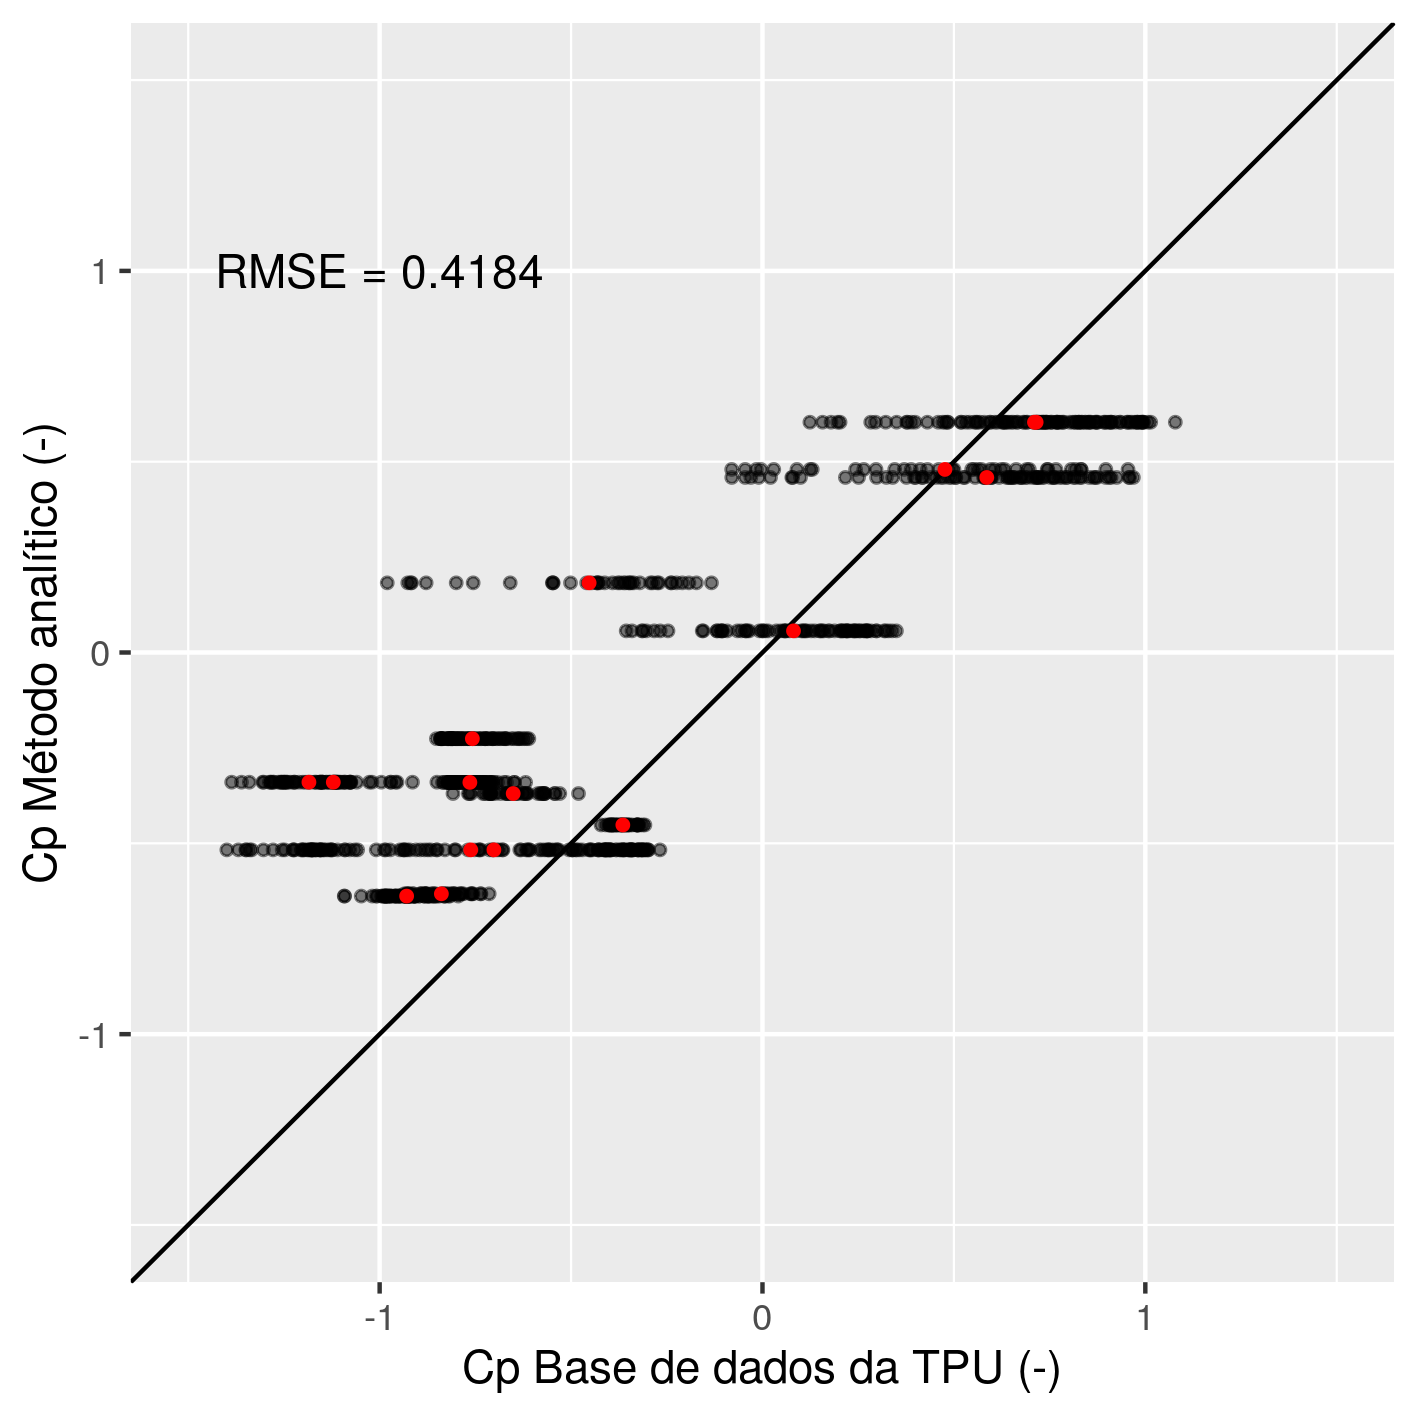
\includegraphics[width=\linewidth]{img/cp_diff_scatter.png}
		%		\caption{Comparação entre os valores de \acrshort{cp} das 25 geometrias}
		\begin{center}
			\small{(b) Geometria de proporções 2:1:2}\\
			\phantom{}		
		\end{center}
	\end{minipage}
	\label{fig:cp_diff_scatter}
\end{figure}

%A partir do resultado da comparação dos \acrshort{cp} nas diferentes geometrias,  
Partindo-se de uma tipologia com proporções de largura, profundidade e altura igual a 2:1:2, as diferenças nos resultados de simulações termoenergéticas com \acrshort{cp} obtidos pelos diferentes métodos foram avaliadas. 
A Figura \ref{fig:cpaverage_ACH_scatter} apresenta a comparação entre as médias anuais de \acrfull{ach}. %, apresentada na ,

\begin{figure}[h]
	\centering
	\caption{Comparação das médias anuais de ACH utilizando-se o método analítico e a base de dados da TPU}
	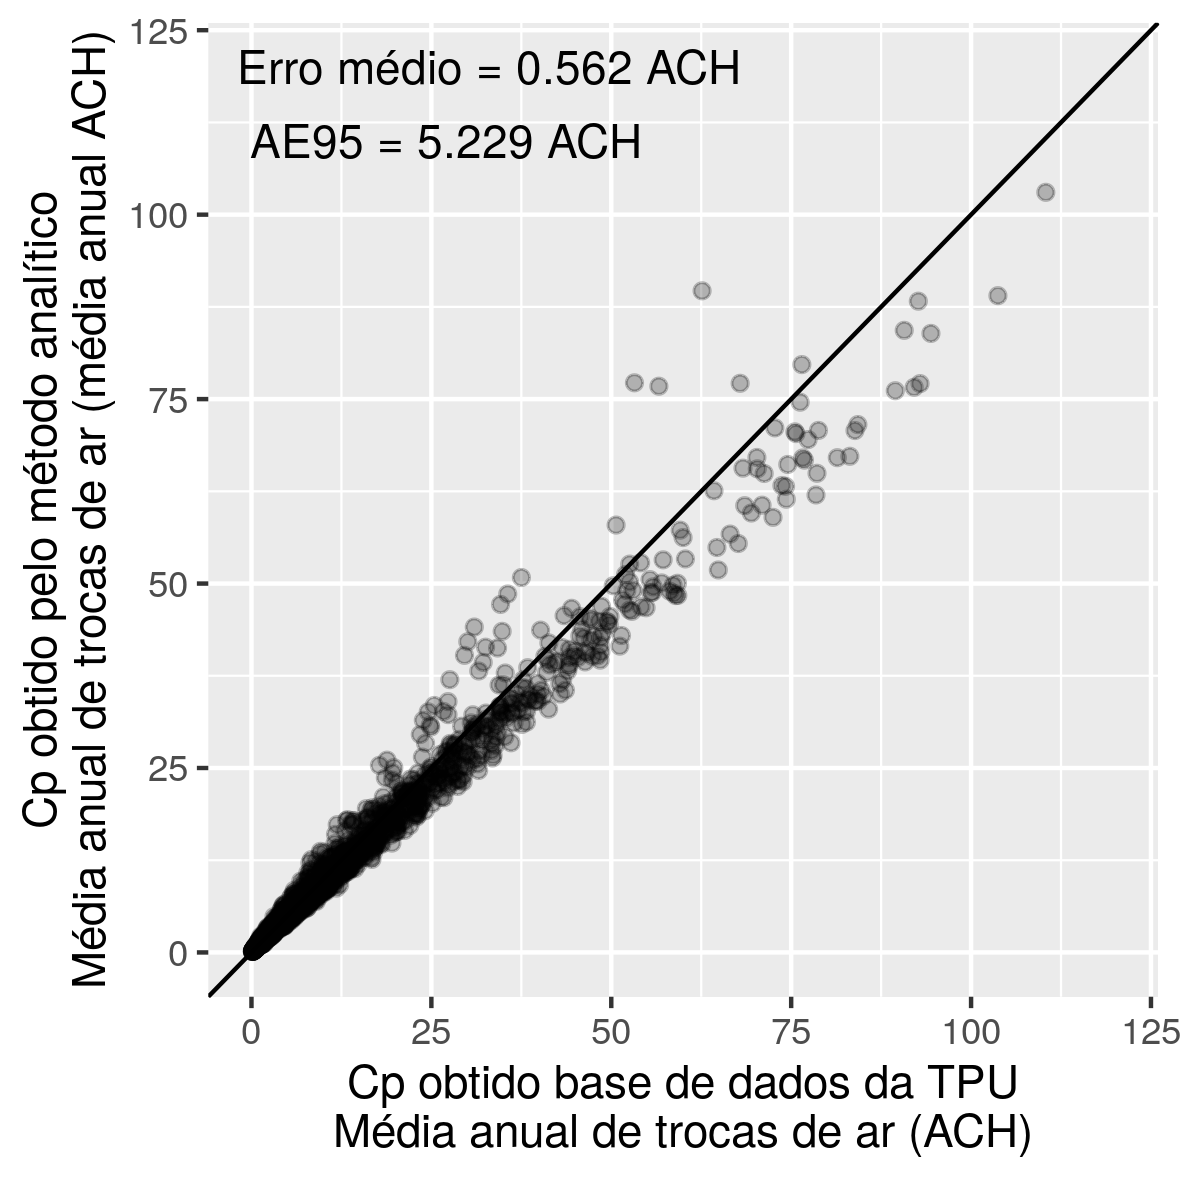
\includegraphics[width=.5\linewidth]{img/cpaverage_ACH_scatter.png}
	\label{fig:cpaverage_ACH_scatter}
	%			\begin{flushleft}
	%				Fonte: o autor.
	%			\end{flushleft}
\end{figure}

A comparação entre as médias anuais de \acrshort{ach} mostra que o \acrlong{ma} faz com que as trocas de ar sejam predominantemente subestimadas nas simulações, possivelmente devido aos menores valores dos \acrshort{cp} obtidos pelo método.
A diferença média foi igual a 0,56 \acrshort{ach}, com o \acrfull{ae95} é igual a 5,23 \acrshort{ach}.

Apesar dessas diferenças nas trocas de ar, a comparação entre as temperaturas operativas médias, apresentada na Figura \ref{fig:cpaverage_tempEHF_scatter}a, mostra que a diferença média da temperatura operativa é 0,04 $^{\circ}$C, sendo que o \acrshort{ae95} é igual a 0,31 $^{\circ}$C.
Essas diferenças são confirmadas como pouco significativas ao se analisar a Figura \ref{fig:cpaverage_tempEHF_scatter}b, com a comparação da \acrfull{ehf}. A média de diferença do \acrshort{ehf} nos casos analisados foi igual a 0,0037, com o \acrshort{ae95} igual a 0,0277.
Portanto, considerou-se que a utilização do \acrlong{ma} para calcular os valores dos \acrshort{cp} é uma alternativa adequada para a simplificação das simulações termoenergéticas.

\begin{figure}[h]
	\centering
	\label{fig:cpaverage_tempEHF_scatter}
	\caption{Comparação de temperaturas operativas e conforto térmico utilizando-se o método analítico e a base de dados da TPU}
	\begin{minipage}{.5\textwidth}
		\centering
		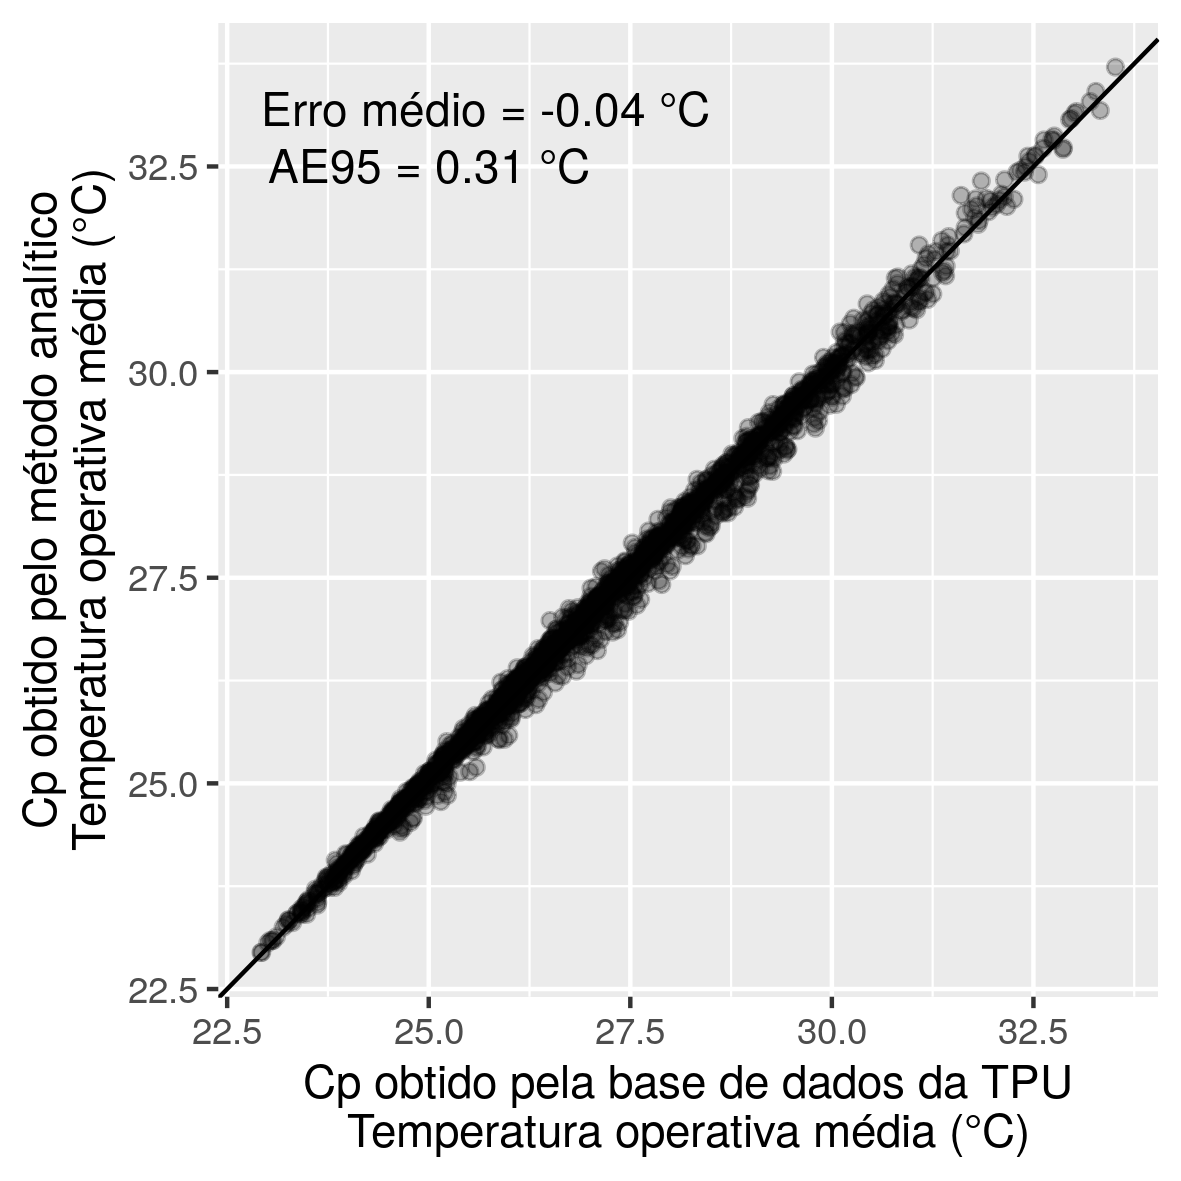
\includegraphics[width=\linewidth]{img/cpaverage_temp_scatter.png}
		%		\caption{Comparação entre os valores de \acrshort{cp} das 25 geometrias}
		\begin{center}
			\small{(a) média anual da temperatura operativa}
		\end{center}
	\end{minipage}%
	\begin{minipage}{.5\textwidth}
		\centering
		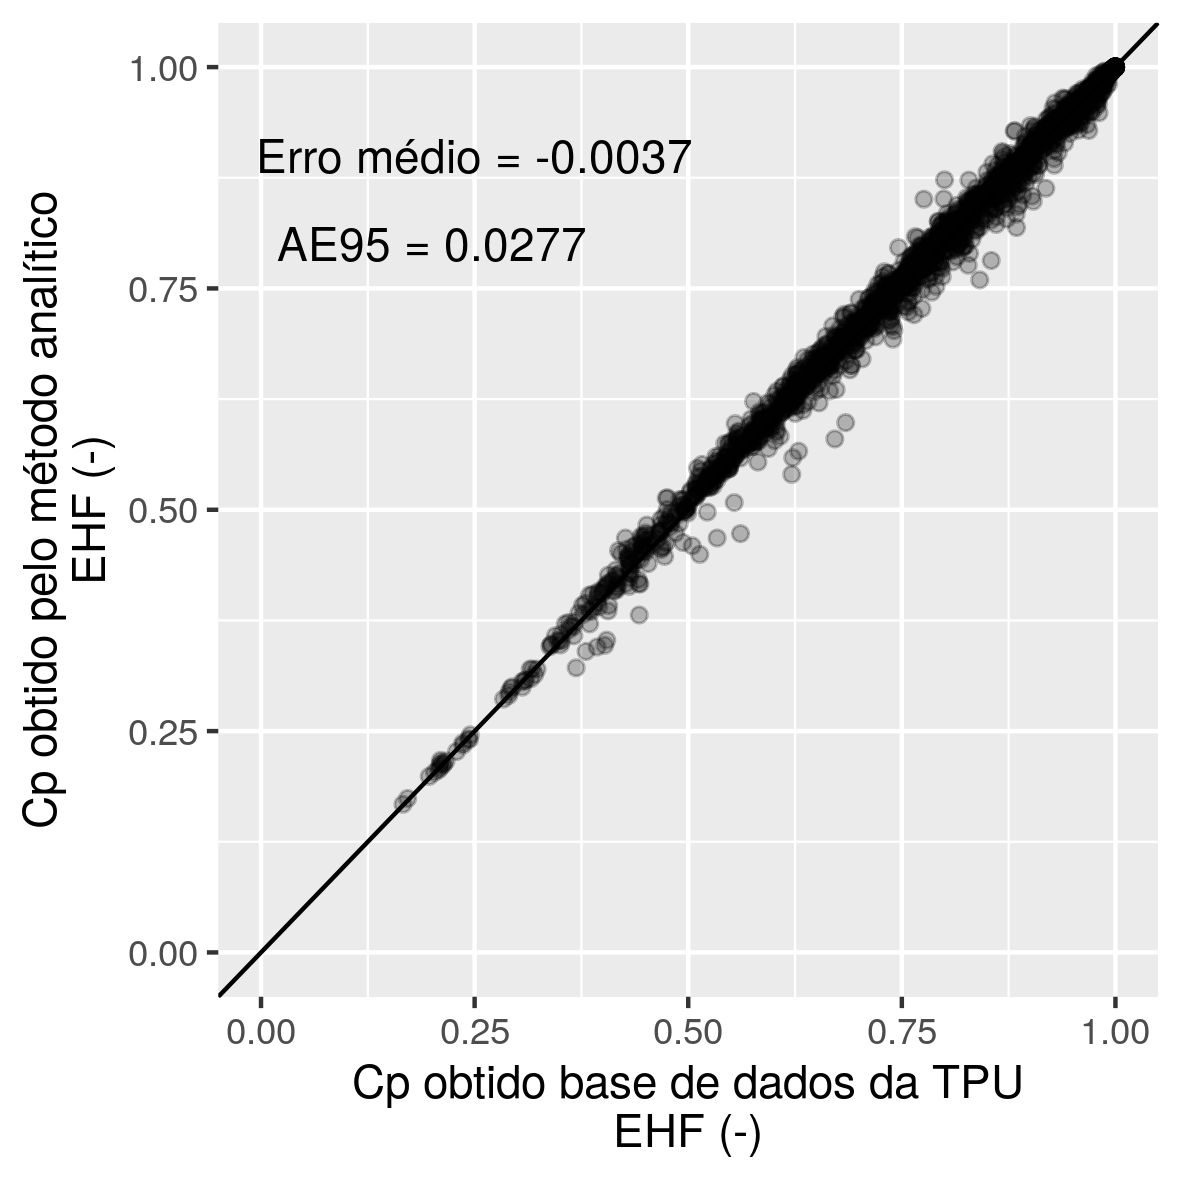
\includegraphics[width=\linewidth]{img/cpaverage_EHF_scatter.png}
		%		\caption{Comparação entre os valores de \acrshort{cp} das 25 geometrias}
		\begin{center}
			\small{(b) \acrlong{ehf}}
		\end{center}
	\end{minipage}
\end{figure}

%\begin{figure}[H]
%	\centering
%	\caption{Comparação entre as médias das temperaturas operativas}
%	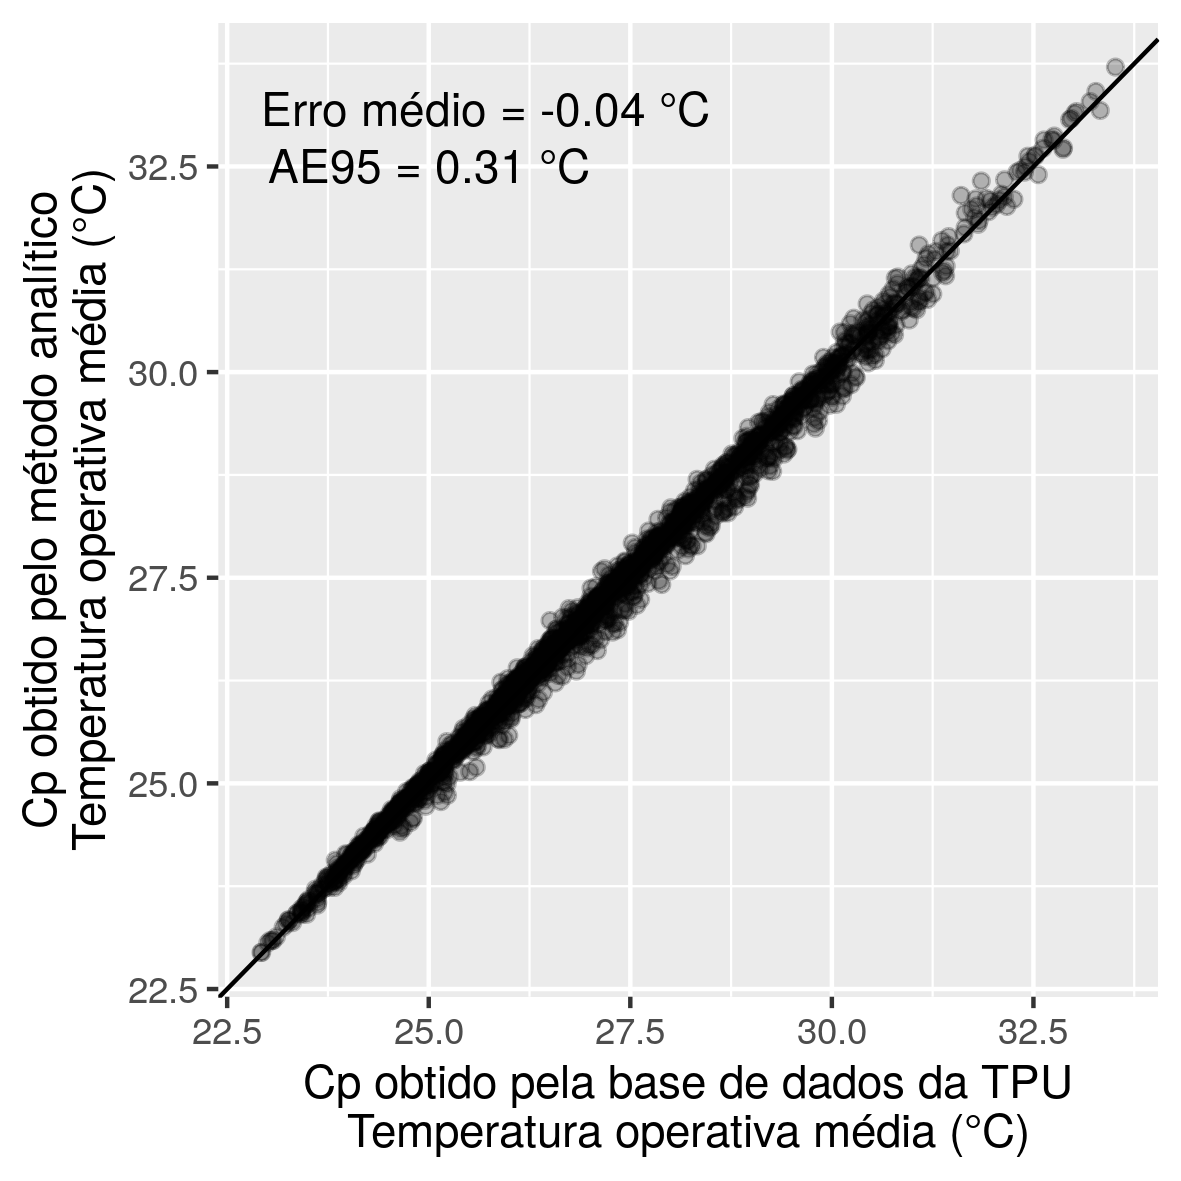
\includegraphics[width=\figsize\linewidth]{img/cpaverage_temp_scatter.png}
%	\label{fig:cpaverage_temp_scatter}
%	%			\begin{flushleft}
%	%				Fonte: o autor.
%	%			\end{flushleft}
%\end{figure}
%
%\begin{figure}[H]
%	\centering
%	\caption{Comparação entre os resultados de EHF}
%	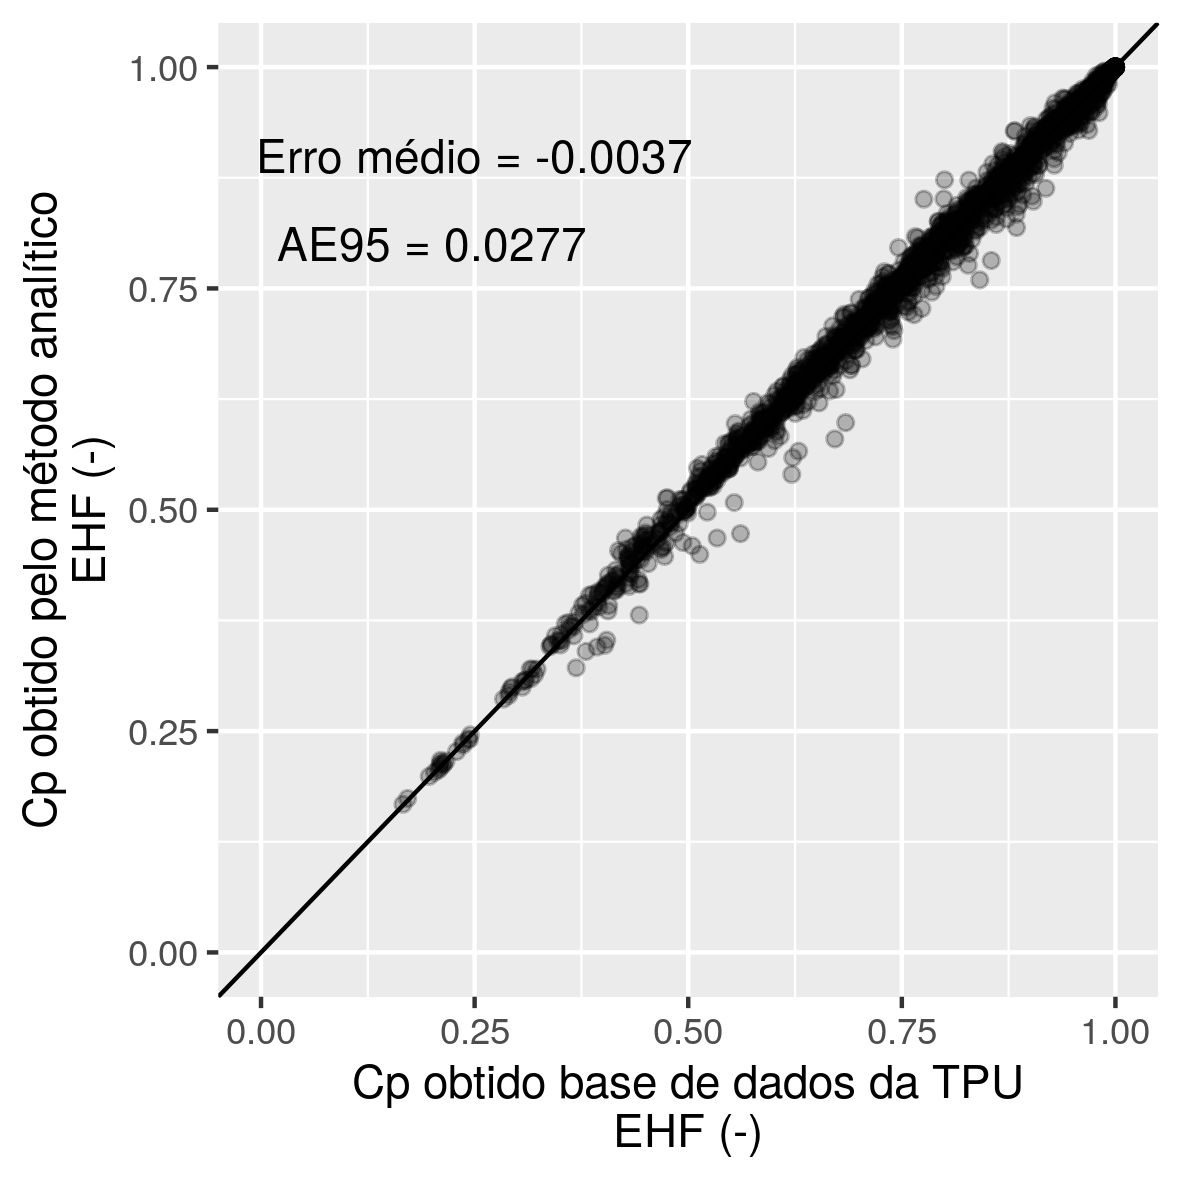
\includegraphics[width=\figsize\linewidth]{img/cpaverage_EHF_scatter.png}
%	\label{fig:cpaverage_EHF_scatter}
%	%			\begin{flushleft}
%	%				Fonte: o autor.
%	%			\end{flushleft}
%\end{figure}

\subsection*{Representação da envoltória com duas camadas}

Os resultados das simulações com as paredes equivalentes subestimaram o \acrshort{ehf} em 0,0107 na média, quando comparados aos resultados das simulações com as paredes de referência. 
Os resultados das simulações para a parede de gesso com isolamento resultaram em um erro médio igual a 0,0099, e um \acrshort{ae95} igual a 0,0304 para o \acrshort{ehf} (Figura \ref{fig:par3_scatter}). O erro absoluto médio foi igual a 0,0100.

\begin{figure}[h]
	\centering
	\caption{Comparação entre os resultados de EHF para a parede de gesso com isolamento}
	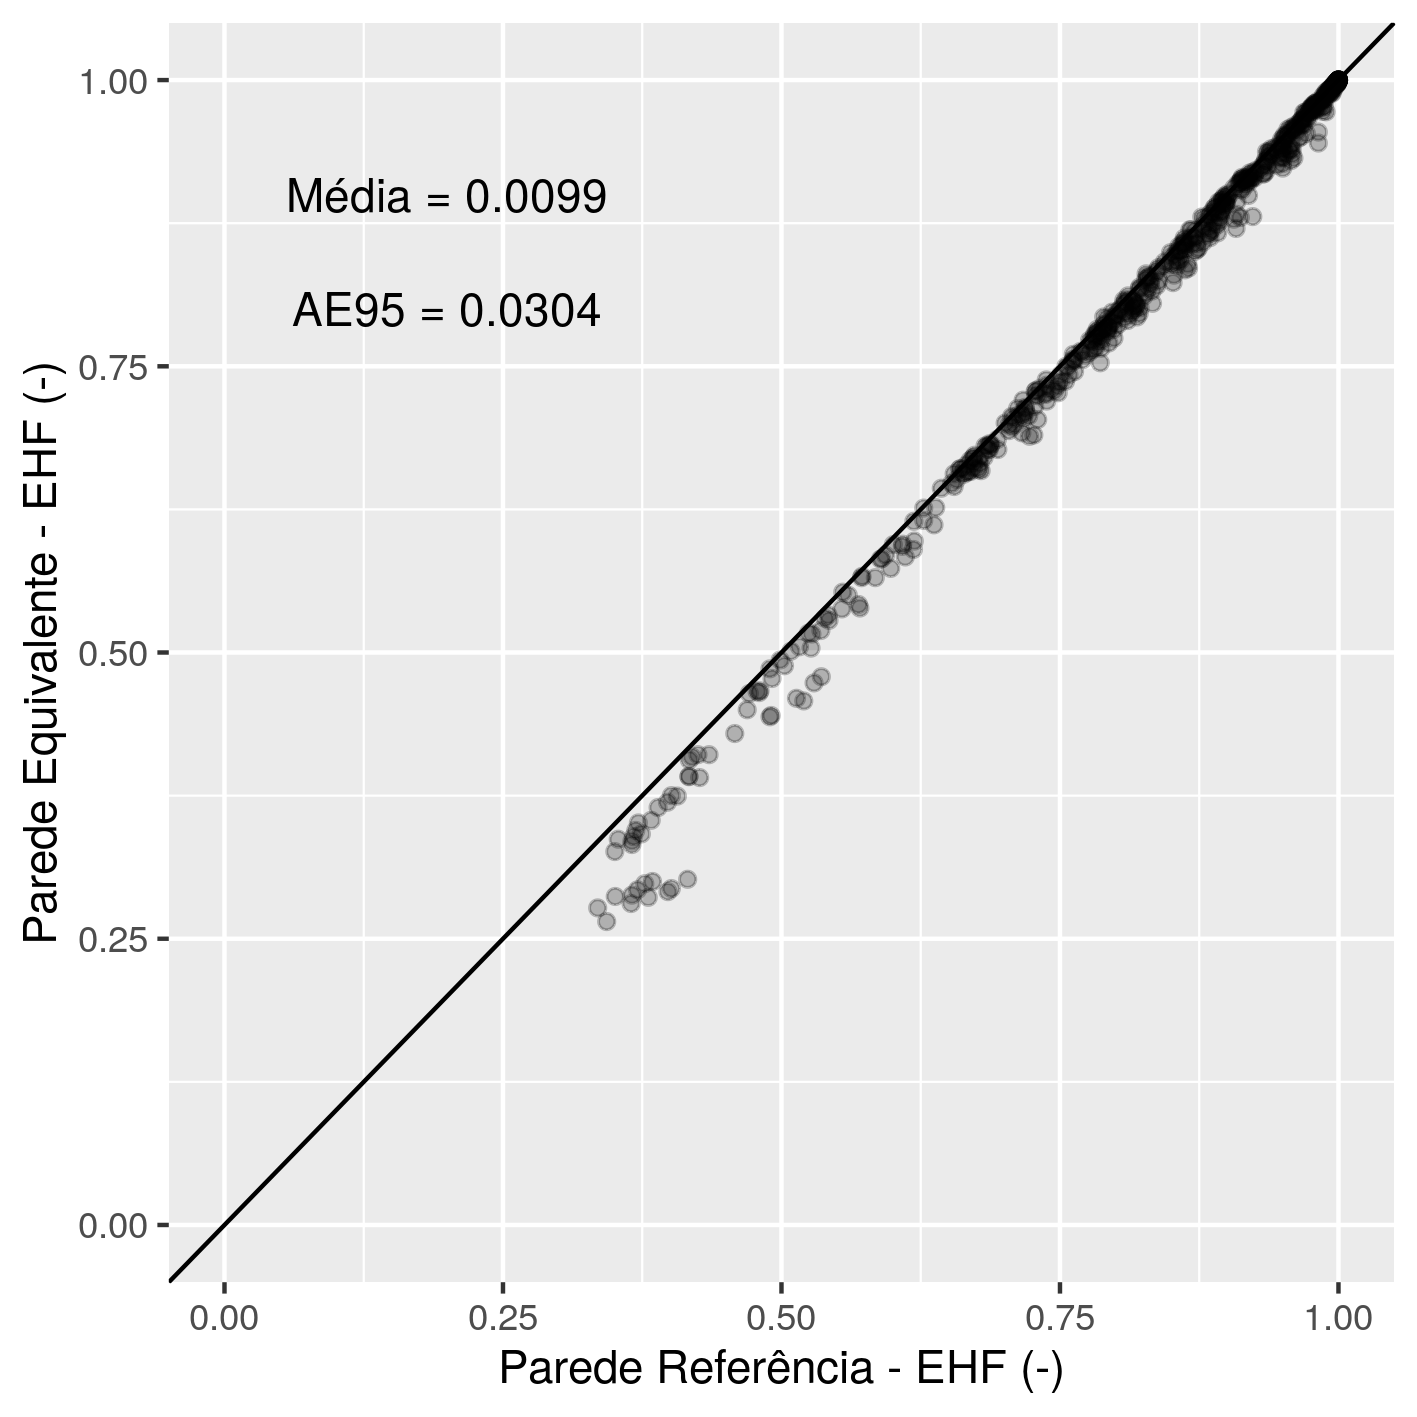
\includegraphics[width=.5\linewidth]{img/paredeeq_EHF_par3_scatter.png}
	\label{fig:par3_scatter}
	%			\begin{flushleft}
	%				Fonte: o autor.
	%			\end{flushleft}
\end{figure}

A representação da parede de alvenaria resultou em comportamentos semelhantes aos da parede de gesso com isoladamente.
Por mais que as diferenças sejam pouco expressivas, observou-se que utilizar o modelo de parede equivalente apresenta-se mais adequado considerando-se apenas metade do valor da \acrfull{ct} da parede. Enquanto que, para a parede equivalente com o valor total da capacidade térmica o erro médio foi igual a 0,0159, o \acrshort{ae95} foi igual a 0,0650, e o erro absoluto médio foi igual a 0,0209 (Figura \ref{fig:par2_scatter}a), para a parede equivalente com a metade do valor da capacidade térmica, o erro médio foi igual a 0,0115, o \acrshort{ae95} foi igual a 0,0604, e o erro absoluto médio foi igual a 0,0189 (Figura \ref{fig:par2_scatter}b).

\begin{figure}[h]
	%	\centering
	\caption{Comparação entre os resultados de EHF para a parede de alvenaria}
	\begin{minipage}{.5\textwidth}
		%		\centering
		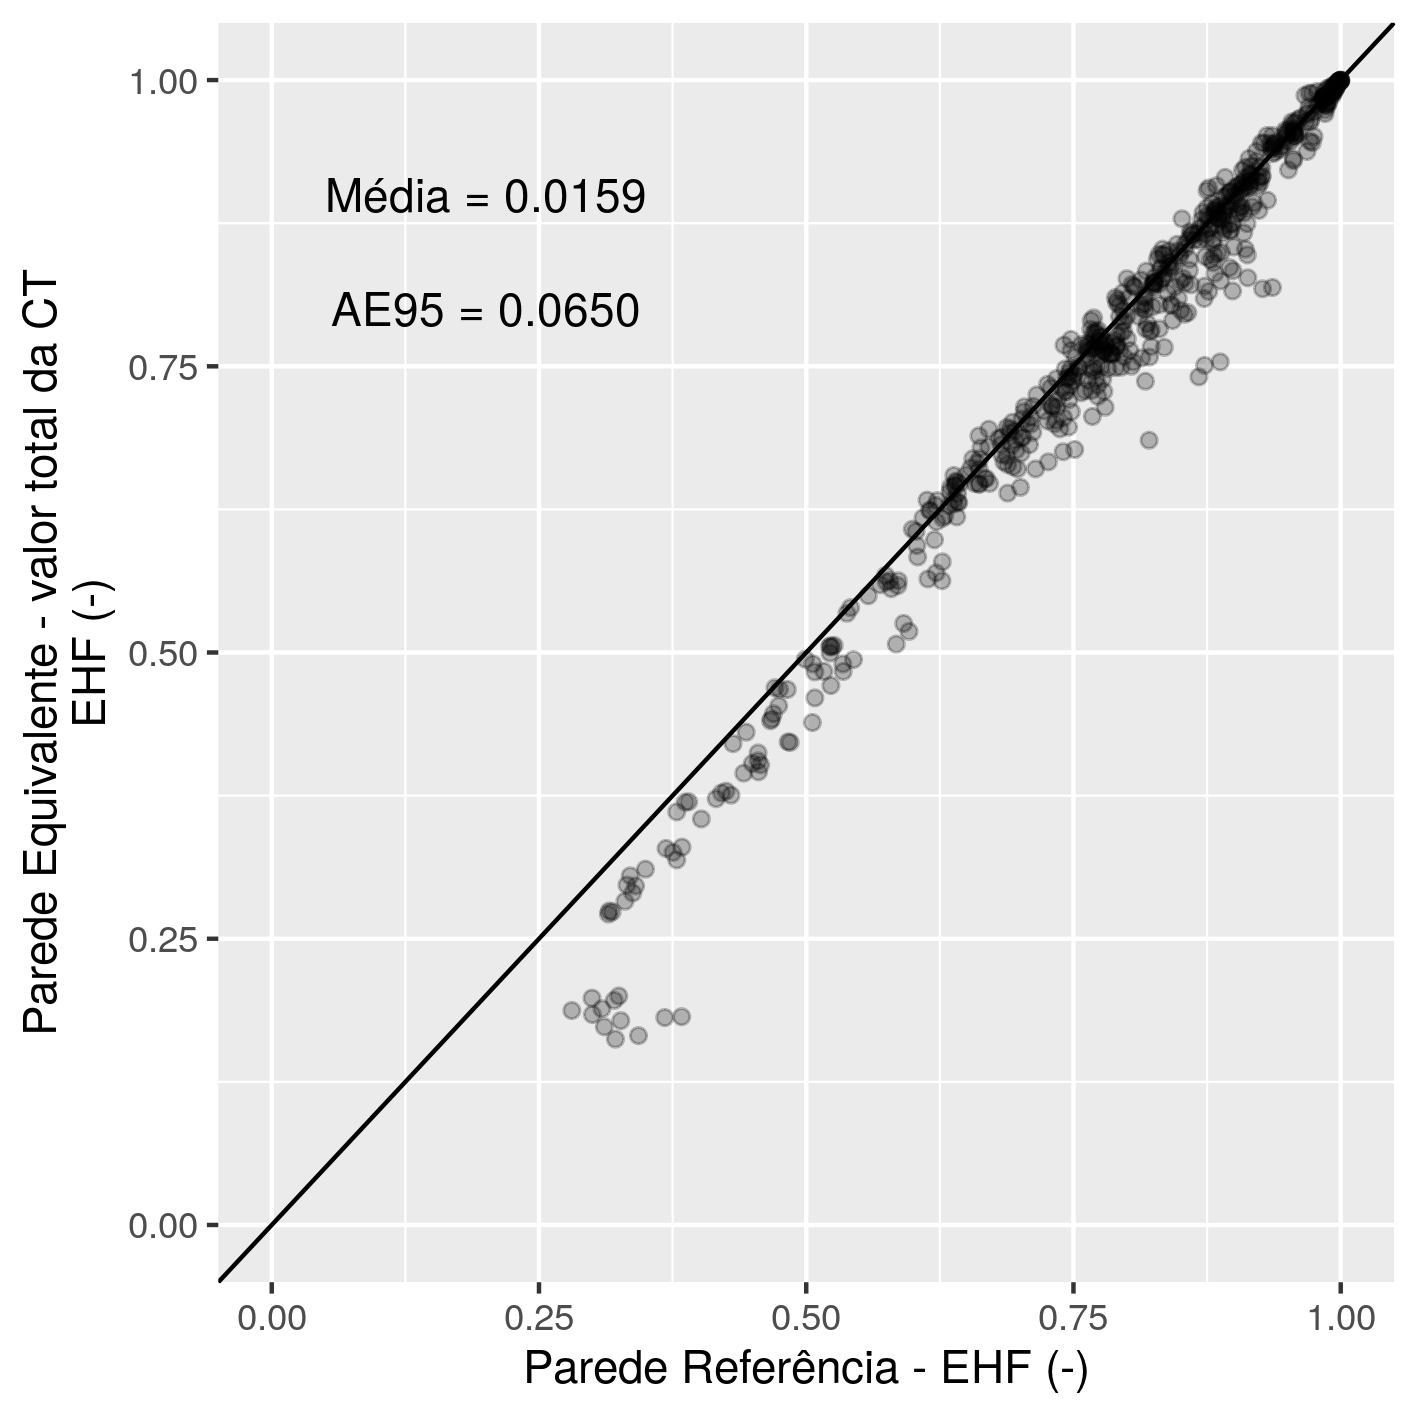
\includegraphics[width=\linewidth]{img/paredeeq_EHF_par2a_scatter.png}
		%		\caption{Comparação entre os valores de \acrshort{cp} das 25 geometrias}
		\begin{center}
			\small{(a) valor total da capacidade térmica}
		\end{center}
	\end{minipage}%
	\begin{minipage}{.5\textwidth}
		%		\centering
		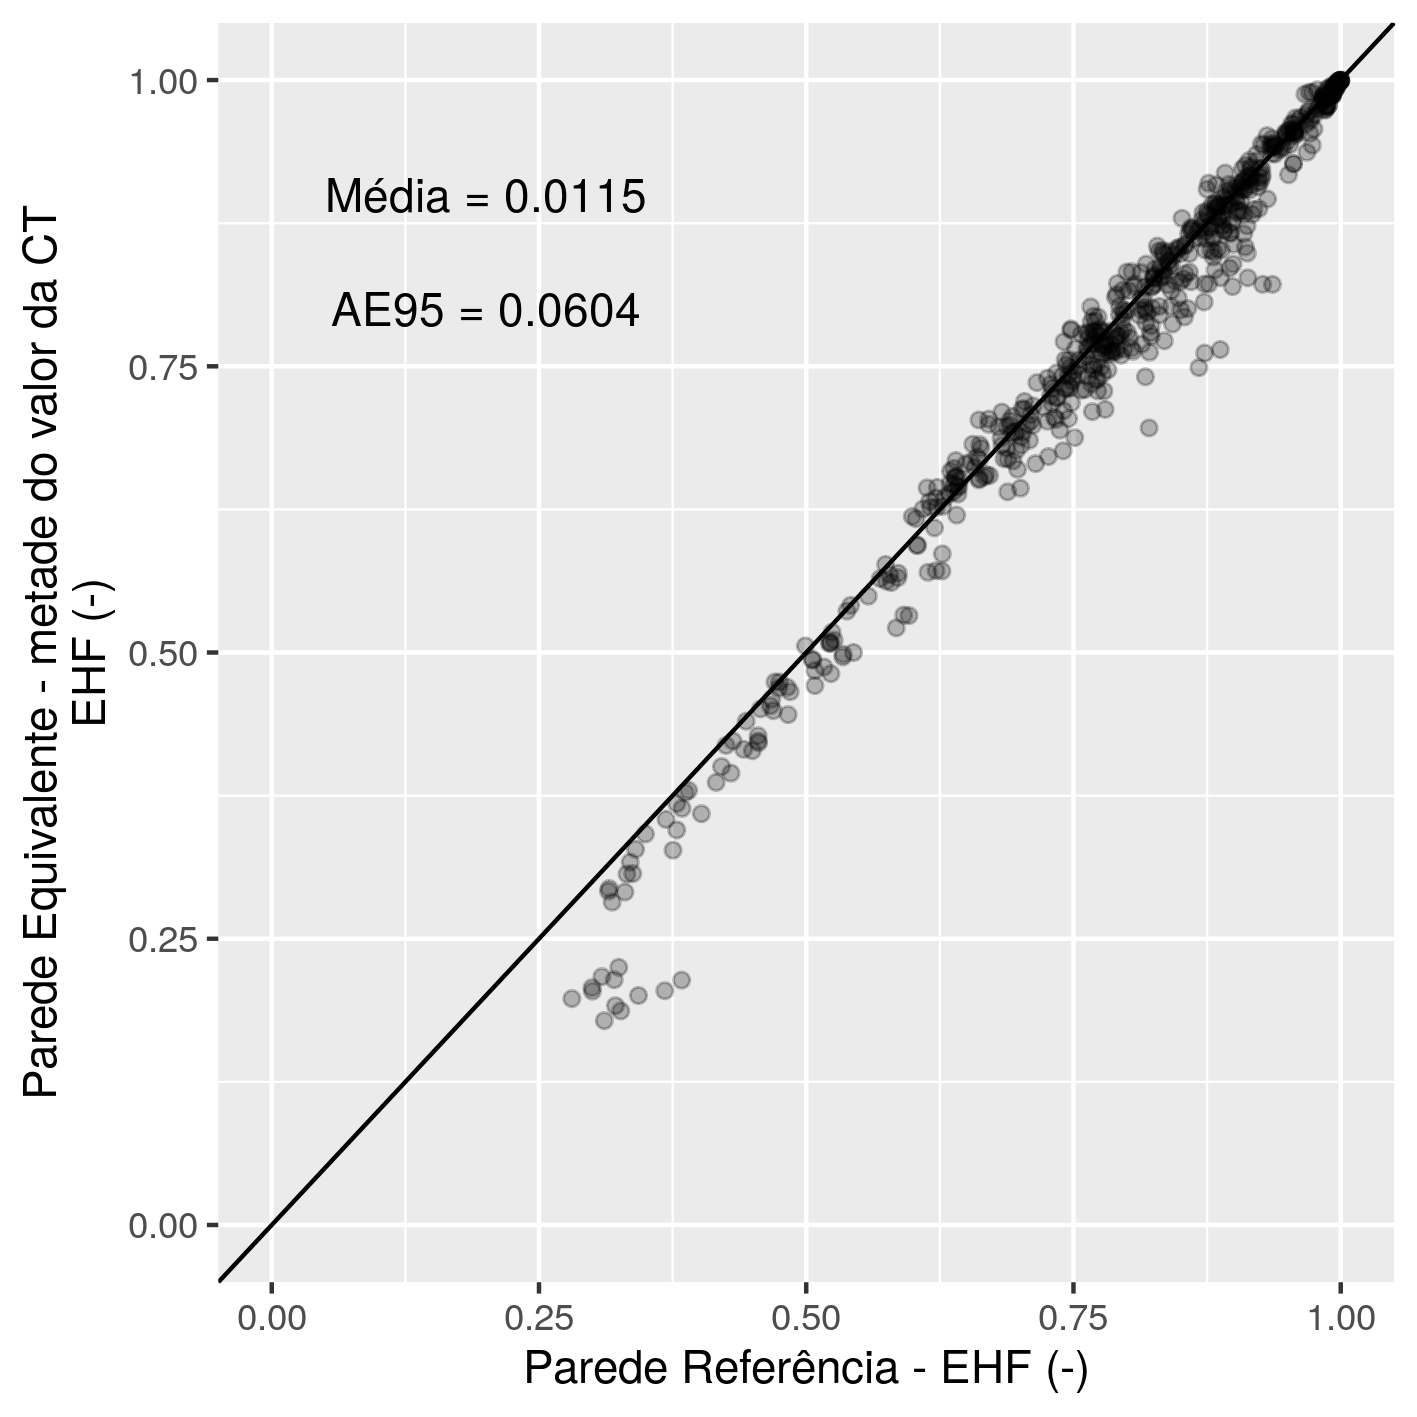
\includegraphics[width=\linewidth]{img/paredeeq_EHF_par2b_scatter.png}
		%		\caption{Comparação entre os valores de \acrshort{cp} das 25 geometrias}
		\begin{center}
			\small{(b) metade do valor da capacidade térmica}\\
			%			\phantom{}		
		\end{center}
	\end{minipage}
	\label{fig:par2_scatter}
\end{figure}

O caso com as maiores diferenças no \acrshort{ehf} foi para uma edificação em contato com o solo, com cobertura exposta, e um fator de abertura da janela igual a 0,23.
Apesar das diferenças nos resultados, o uso da parede equivalente facilita a parametrização da transmitância térmica e da capacidade térmica. Por esse motivo, considerou-se as diferenças pouco significativas, e a parede equivalente foi adotada para simplificar as simulações.

\subsection*{Condição de contorno das paredes adjacentes à edificação}

A simplificação das simulações adotando-se apenas uma zona térmica foi avaliada para duas condições de contorno. Os resultados mostram que a maneira mais adequada de representar as paredes adjacentes à circulação da edificação é considerando-as como adiabáticas (sem trocas de calor pela superfície).
Considerar as paredes adjacentes à circulação como \textit{Outdoors} (voltada para o lado externo, sem incidência de radiação solar ou vento), faz com que os resultados do \acrshort{ehf} sejam subestimados em 0,0868 em média, como \acrshort{ae95} igual a 0,1865 (Figura \ref{fig:szout}a).
Os resultados das simulações considerando-se as paredes voltadas para o corredor como adiabáticas subestimaram o \acrshort{ehf} em 0,0051 na média, como \acrshort{ae95} igual a 0,0804 (Figura \ref{fig:szout}b).

\begin{figure}[h]
	\caption{Comparação entre os resultados de EHF para diferentes condições de contorno das paredes}
	\begin{minipage}{.5\textwidth}
		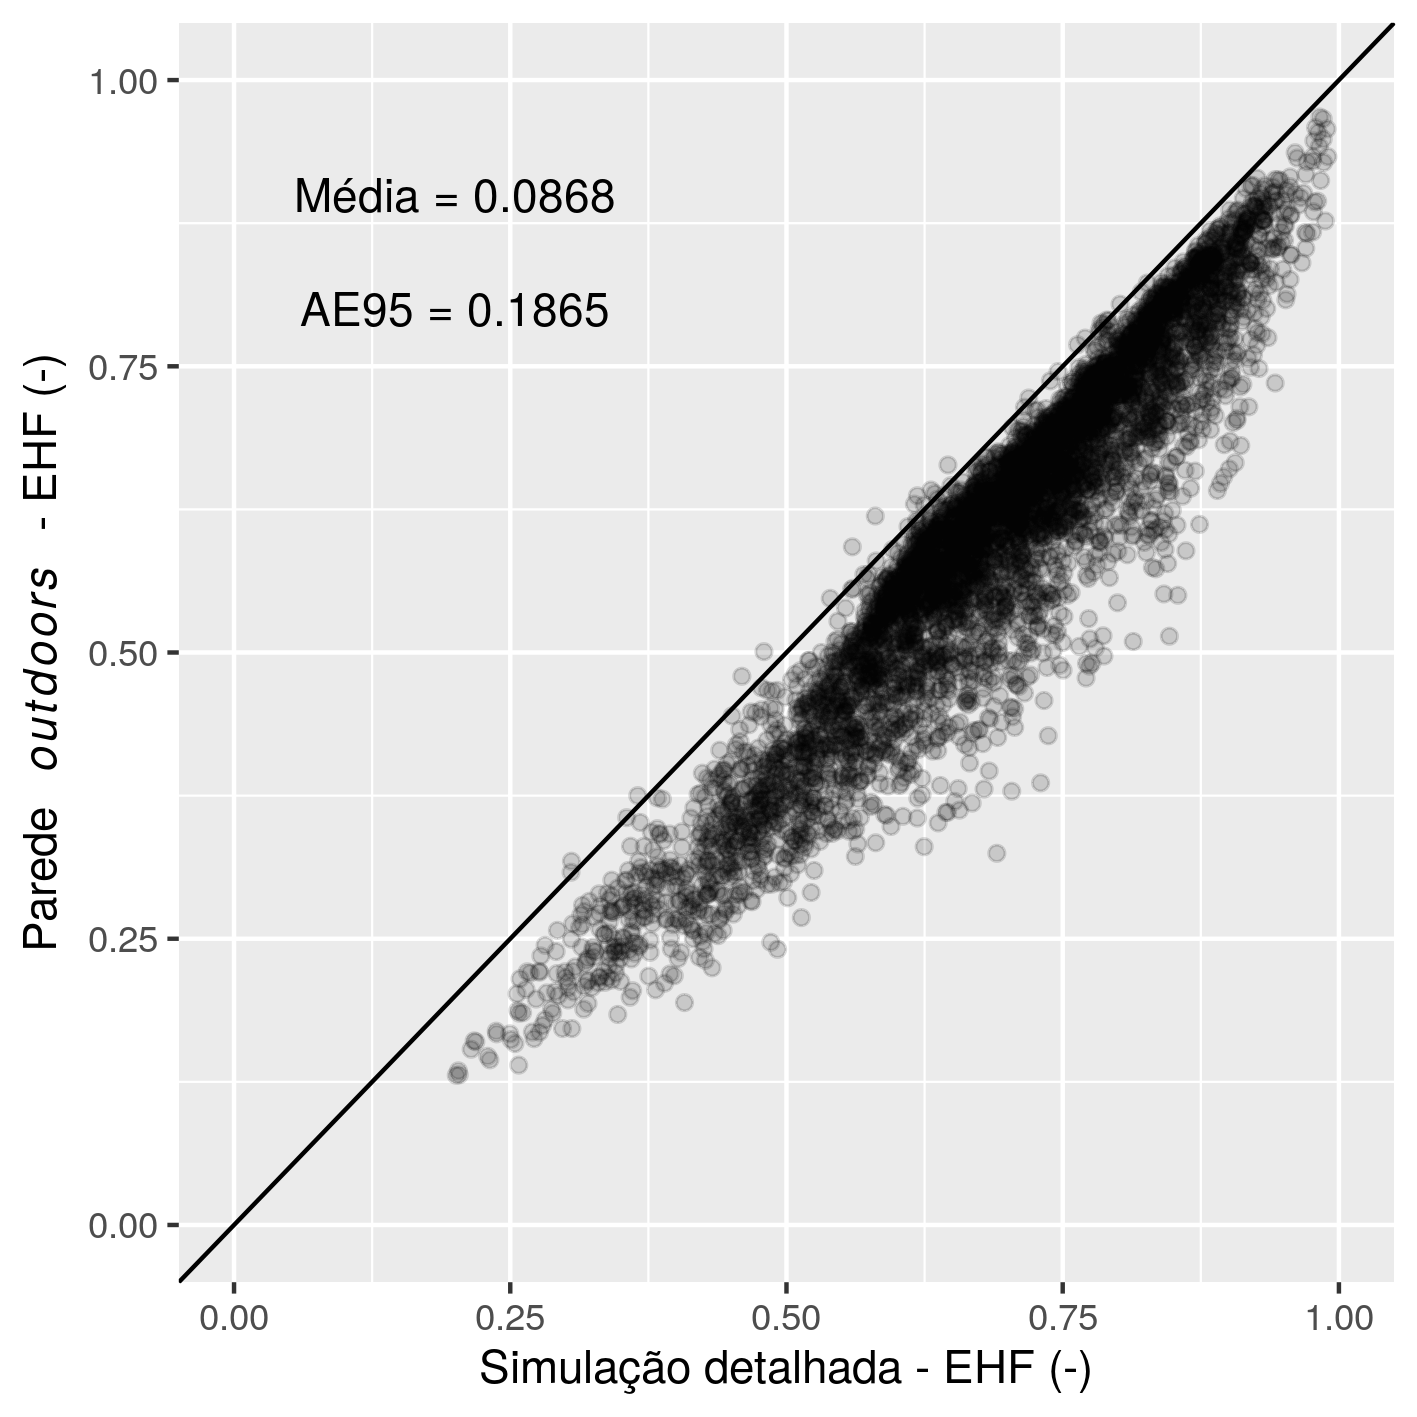
\includegraphics[width=\linewidth]{img/szout_EHF_scatter.png}
		\begin{center}
			\small{(a) \textit{Outdoors}}
		\end{center}
	\end{minipage}%
	\begin{minipage}{.5\textwidth}
		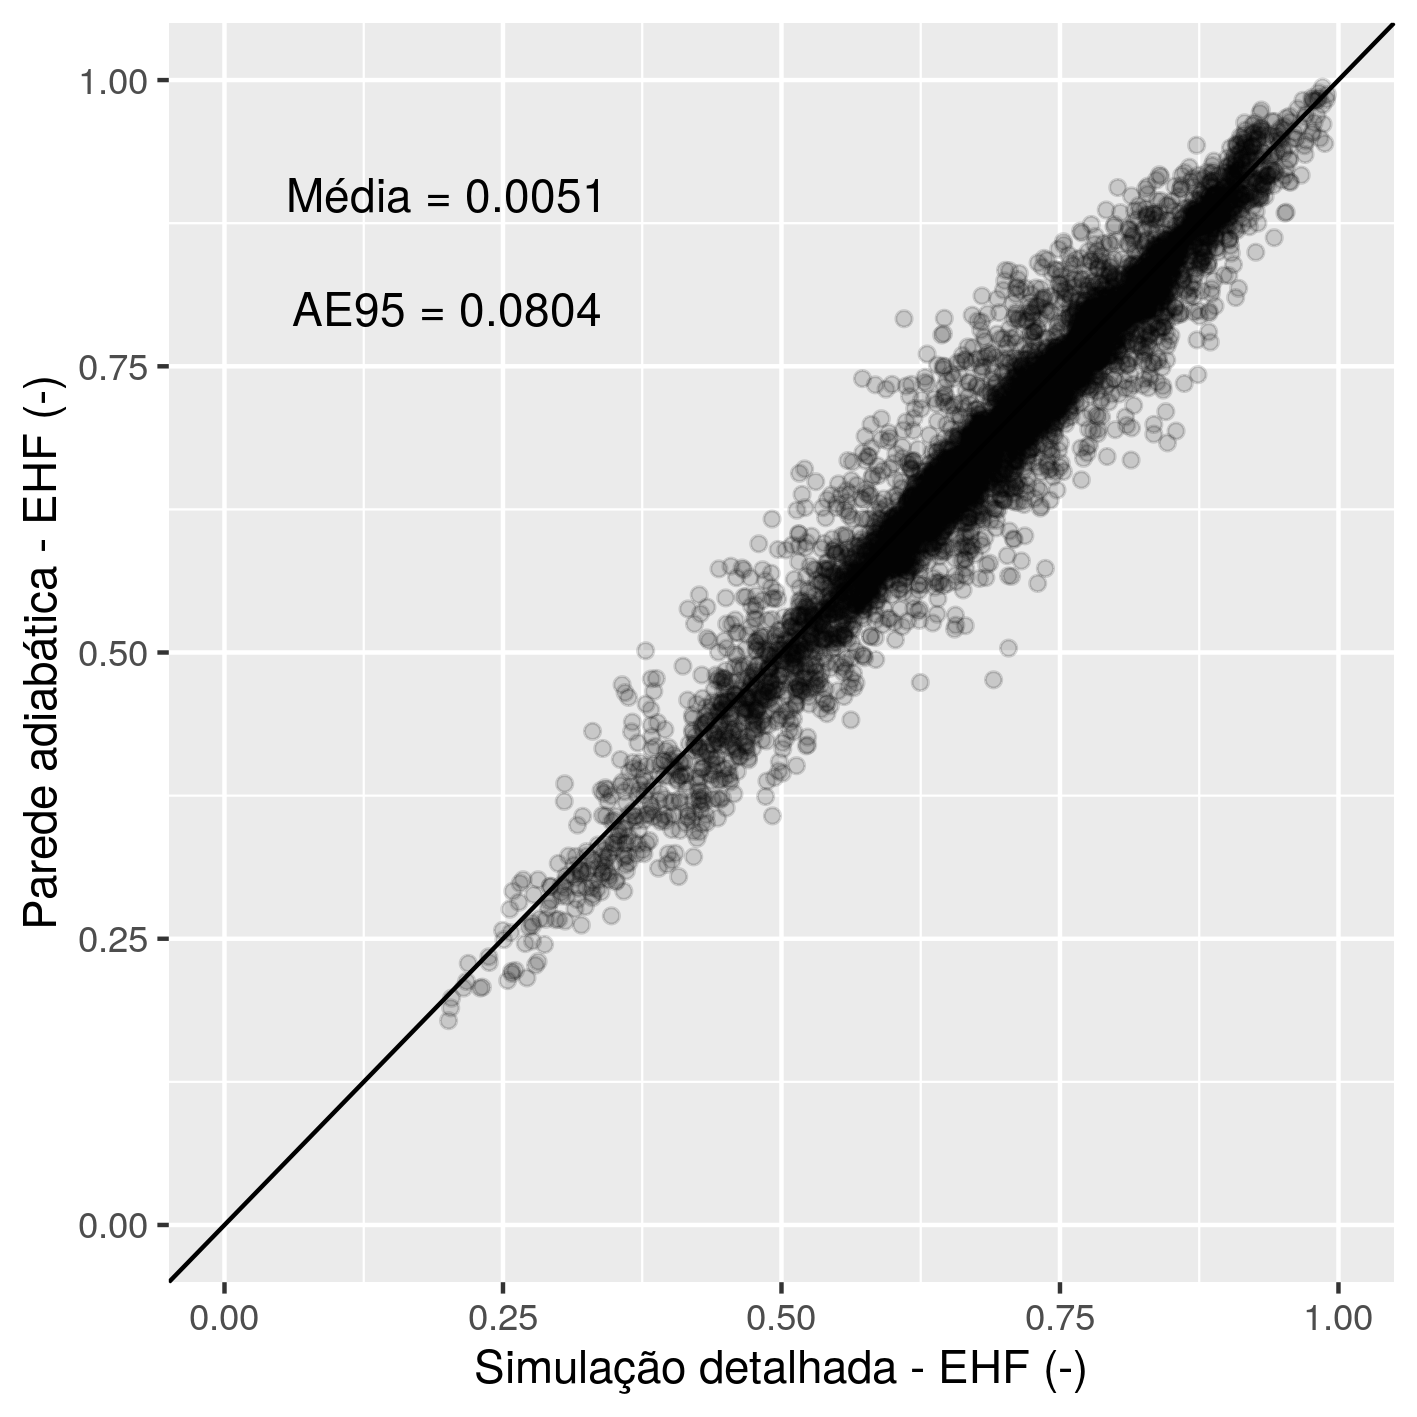
\includegraphics[width=\linewidth]{img/szadi_EHF_scatter.png}
		\begin{center}
			\small{(b) Adiabática}\\
			%			\phantom{}		
		\end{center}
	\end{minipage}
	\label{fig:szout}
\end{figure}

%\begin{figure}[H]
%	\centering
%	\caption{Comparação entre os resultados de EHF para parede \textit{Outdoors}}
%	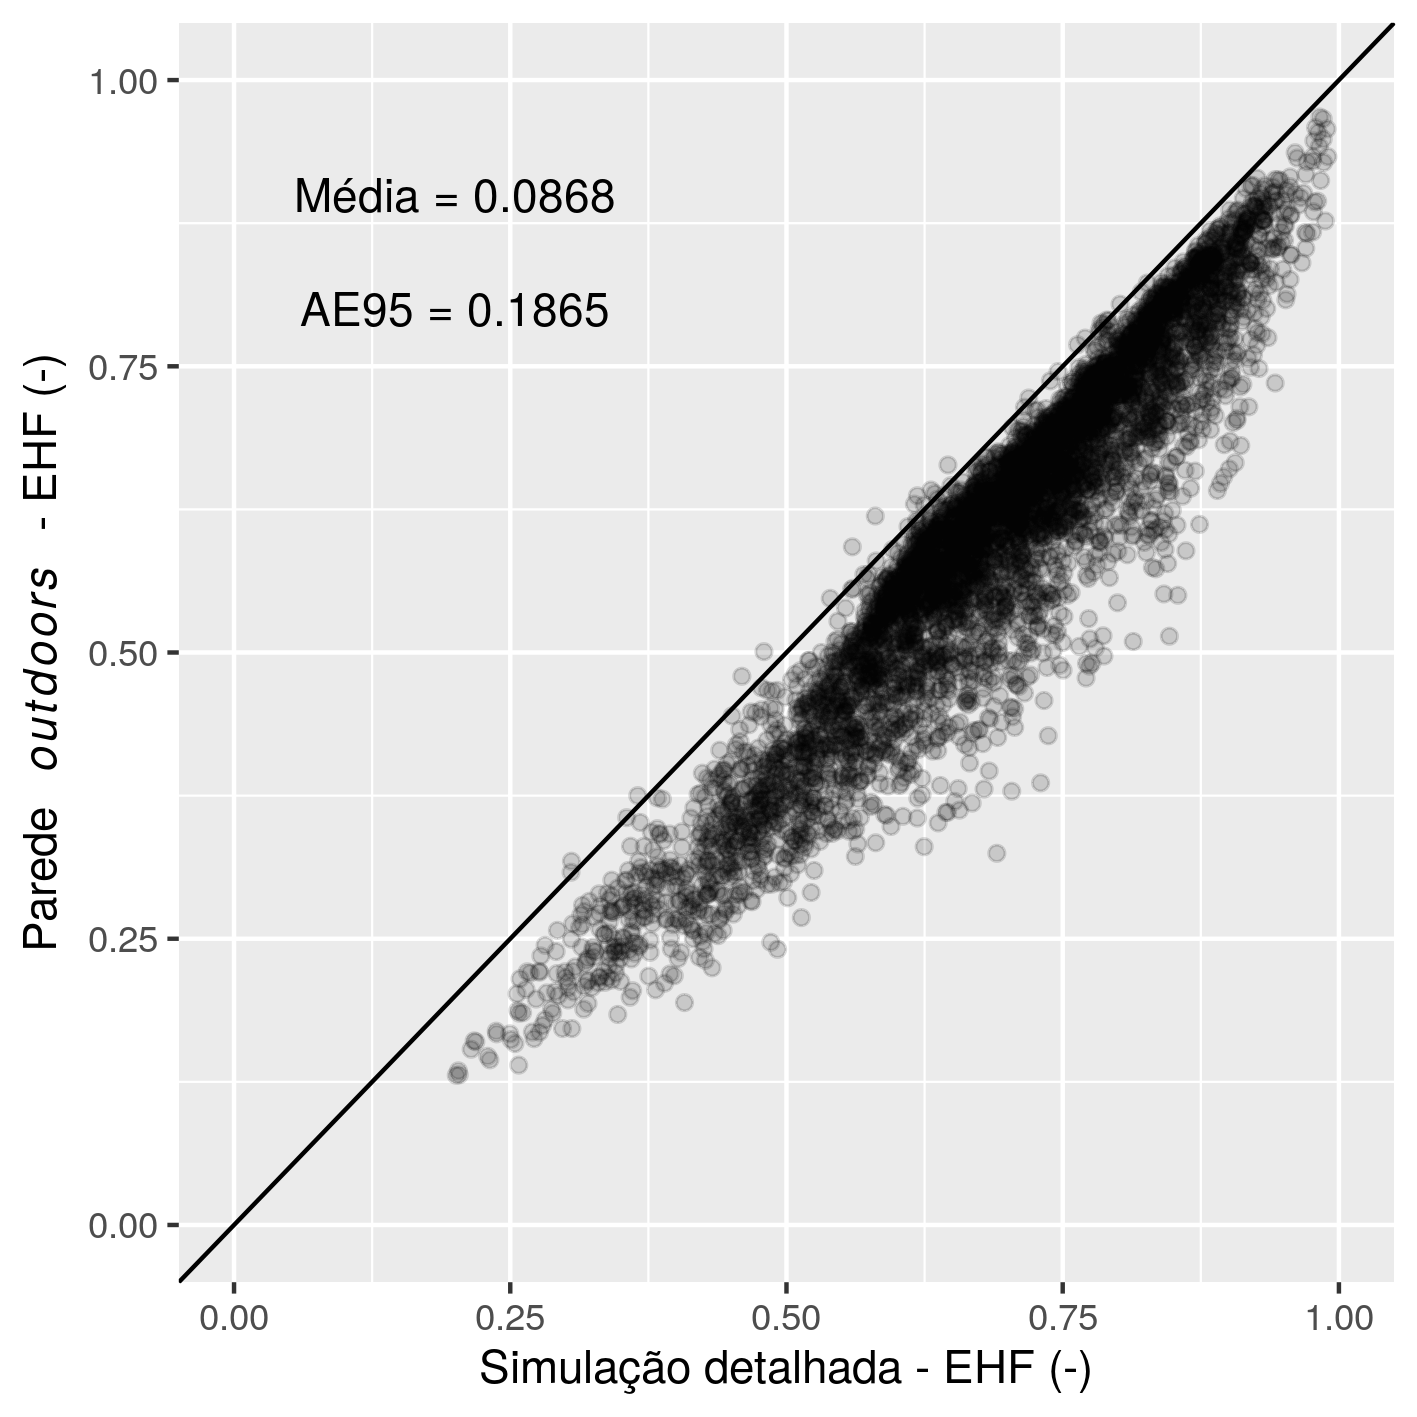
\includegraphics[width=1\linewidth]{img/szout_EHF_scatter.png}
%	\label{fig:szout_EHF}
%	%			\begin{flushleft}
%	%				Fonte: o autor.
%	%			\end{flushleft}
%\end{figure}

%\begin{figure}[H]
%	\centering
%	\caption{Comparação entre os resultados de EHF para parede adiabática}
%	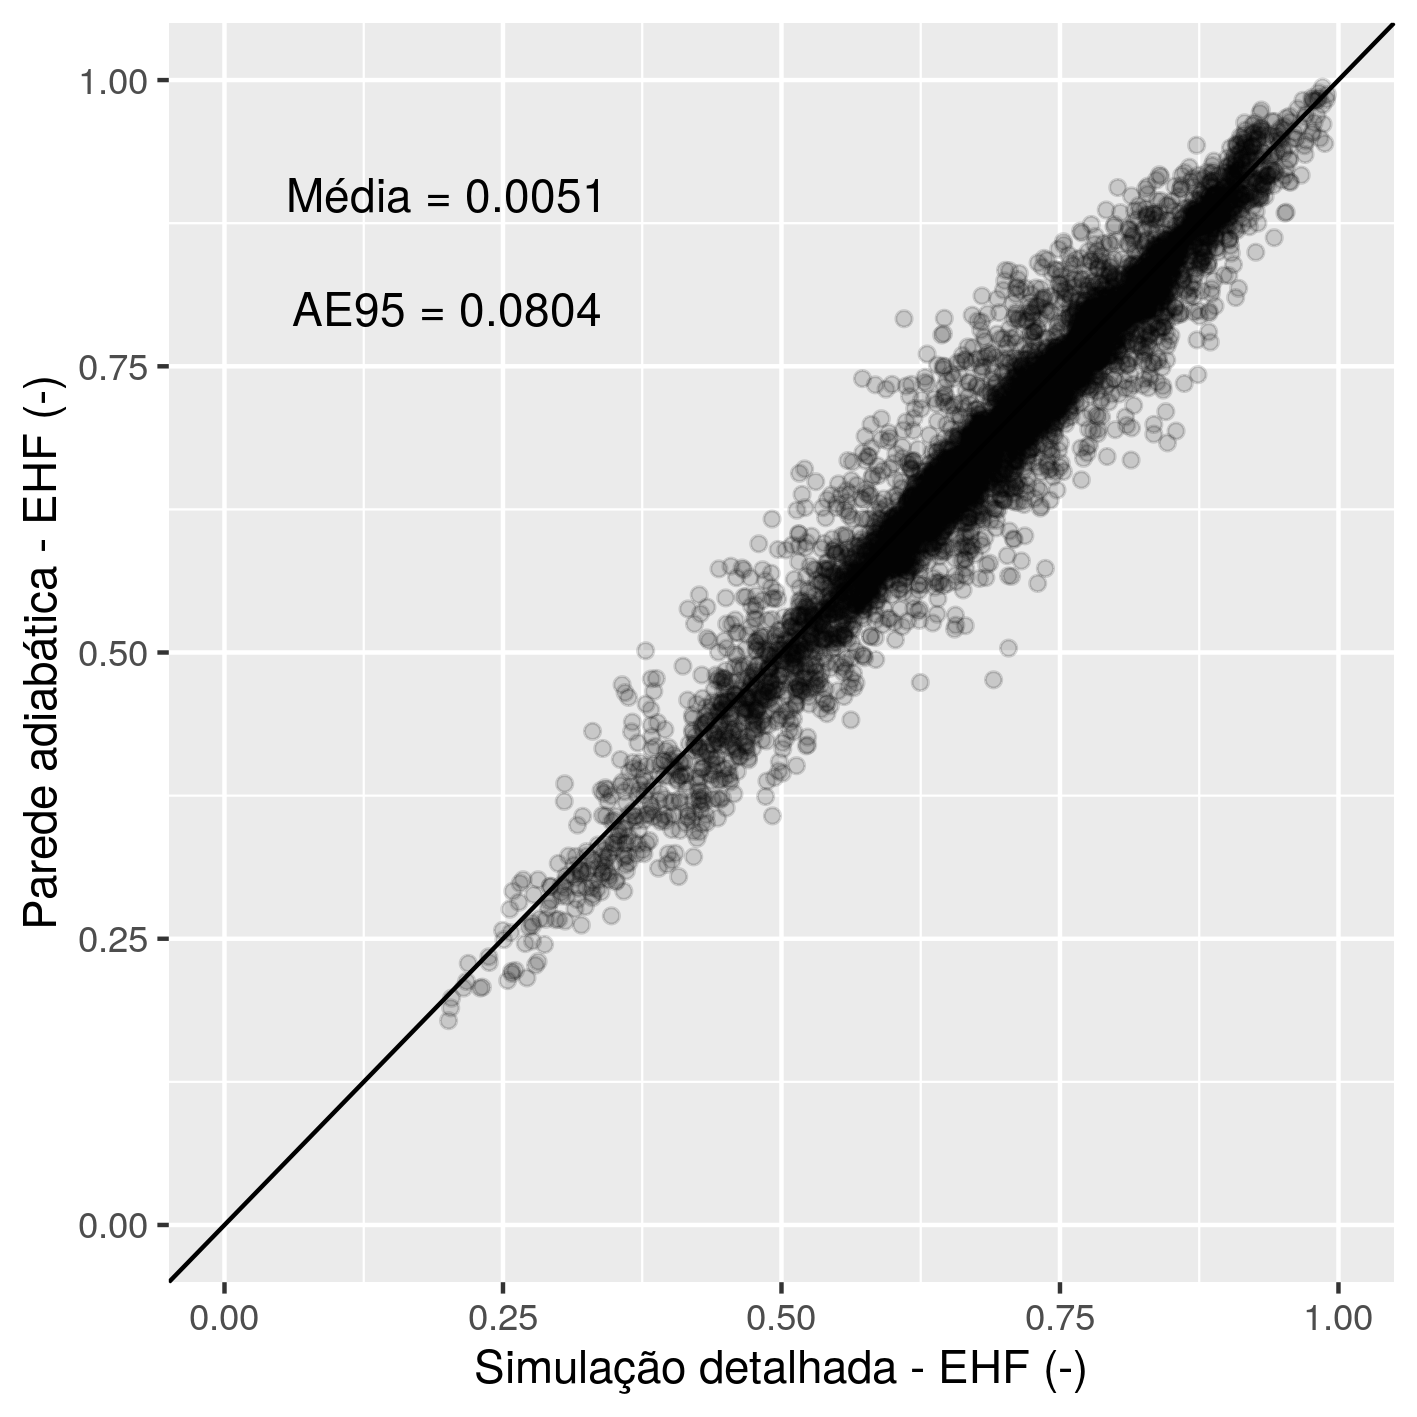
\includegraphics[width=1\linewidth]{img/szadi_EHF_scatter.png}
%	\label{fig:szadi_EHF}
%	%			\begin{flushleft}
%	%				Fonte: o autor.
%	%			\end{flushleft}
%\end{figure}

A partir dos resultados obtidos, definiu-se as paredes voltadas para a circulação como adiabáticas no desenvolvimento das simulações simplificadas.

\subsection*{Modelagem da ventilação natural na simulação simplificada}

Nesta etapa do trabalho, as simulações foram conduzidas para se obter duas respostas:
(1) se é adequado o uso do \acrfull{cpeq} para ser associado à porta da zona térmica; (2) qual deveria ser o coeficiente de vazão mássica de ar adotado para o objeto \textit{AirflowNetwork:MultiZone:Surface:Crack}.

Para analisar simultaneamente o desempenho do $Cp_{eq}$ e dos coeficientes de vazão mássica de ar, o gráfico da Figura \ref{fig:pareto} foi gerado, observando-se as raízes dos erros médios quadráticos (\acrshort{rmse}).
%É possível observar que as simulações desenvolvidas utilizando-se o $Cp_{eq}$ obtiveram resultados com \acrshort{rmse} menores do que as simulações desenvolvidas utilizando-se o \acrshort{cp} obtido diretamente pelo \acrlong{ma}.
Para a definir o coeficiente de vazão mássica de ar, levou-se em conta, inicialmente, as diferenças relacionadas ao \acrshort{ach}, observando-se suas médias anuais.
No entanto, valores iguais de médias anuais não garante que os resultados de \acrshort{ach} sejam iguais nos mesmos \textit{timesteps} das simulações. Como os \acrshort{rmse} relacionados ao \acrshort{ach} eram semelhantes entre si, e o desenvolvimento das simulações é voltado para obter a maior exatidão possível para os resultados de \acrshort{ehf}, optou-se por definir o coeficiente de vazão mássica de ar com valor igual a 0,1 kg/sPa$^n$ em 1 Pa, pois as simulações desenvolvidas utilizando-se este valor resultaram nos menores erros de \acrshort{ehf}.

\begin{figure}[h]
	\centering
	\caption{Análise relacionada ao RMSE do EHF e do ACH médio}
	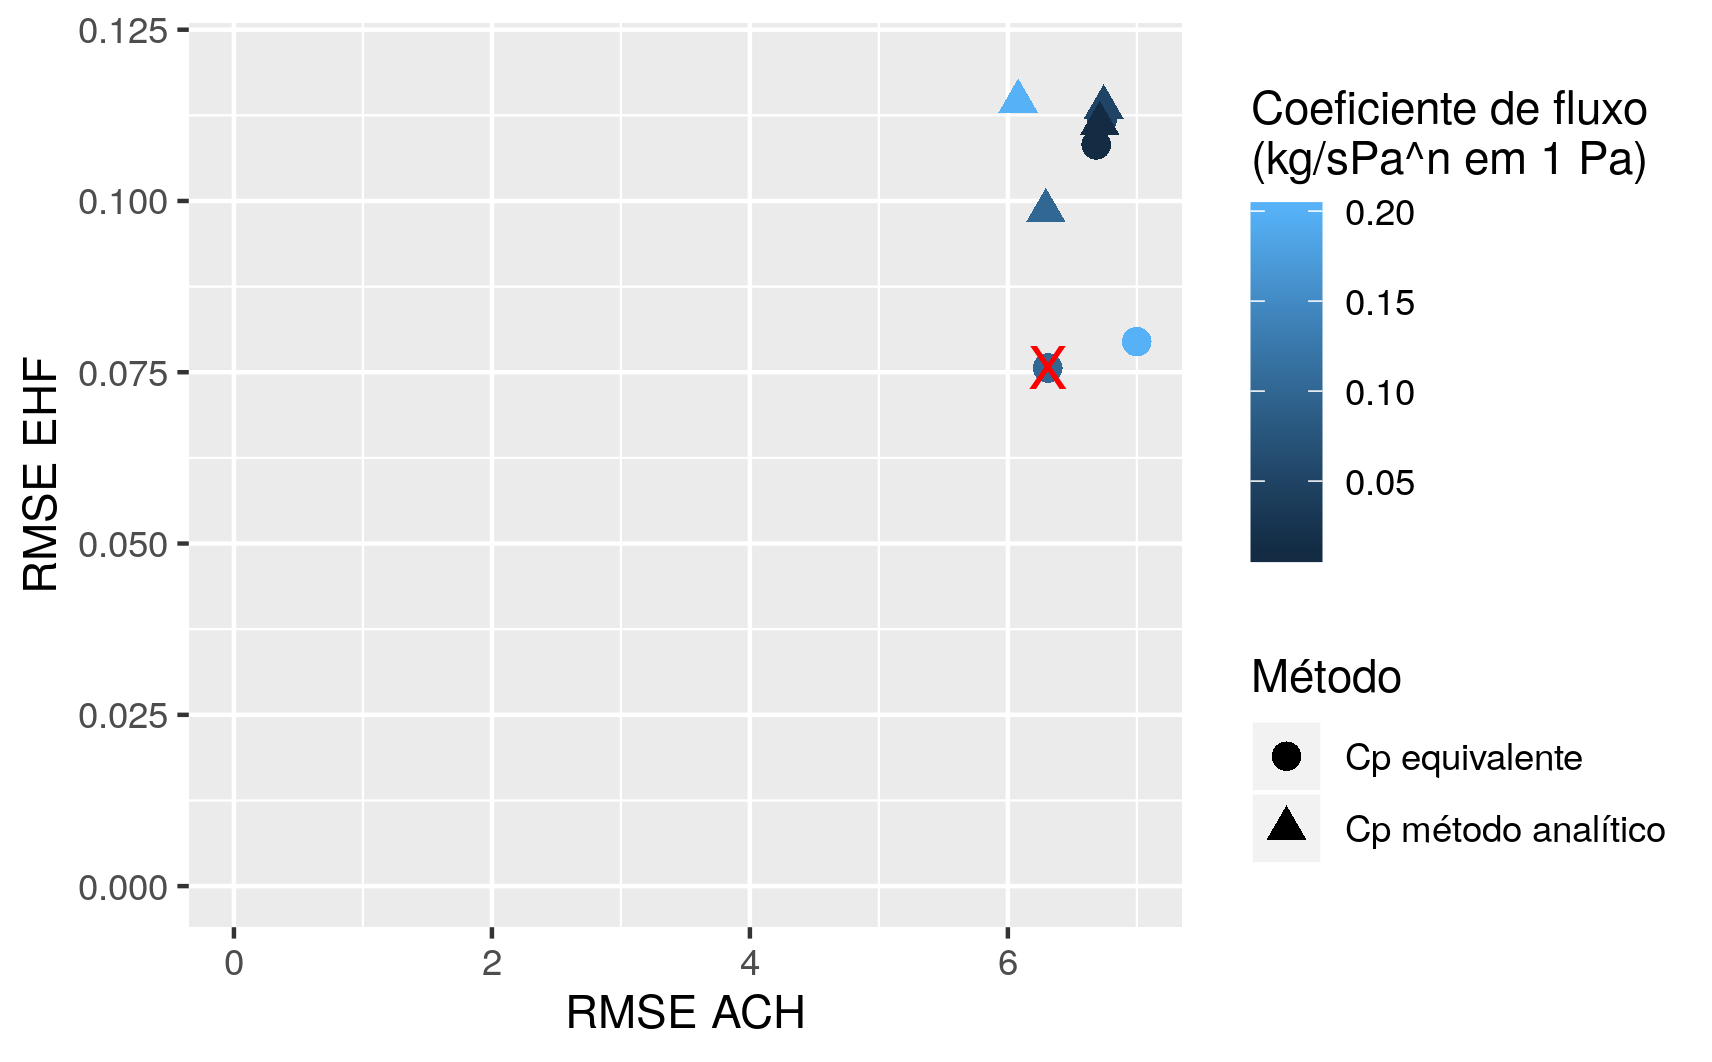
\includegraphics[width=.9\linewidth]{img/cpeq_pareto_fixed.png}
	\label{fig:pareto}
	%			\begin{flushleft}
	%				Fonte: o autor.
	%			\end{flushleft}
\end{figure}

Na Figura \ref{fig:pareto}, o ponto do coeficiente de vazão mássica de ar com valor a 0,1 kg/sPa$^n$ em 1 Pa está destacado com um "X".
A Figura \ref{fig:crack01} apresenta a comparação dos resultados de \acrshort{ach} e \acrshort{ehf} obtidos pelas simulações detalhadas, comparados aos resultados obtidos pela simulação simplificada, utilizando-se o coeficiente de vazão mássica de ar adotado, com valor igual 0,1 kg/sPa$^n$ em 1 Pa.

\begin{figure}[h]
	\caption{Comparação entre os resultados de ACH e EHF para coeficiente de vazão mássica de ar com valor igual 0,1 kg/sPa$^n$ em 1 Pa}
	\begin{minipage}{.5\textwidth}
		\centering
		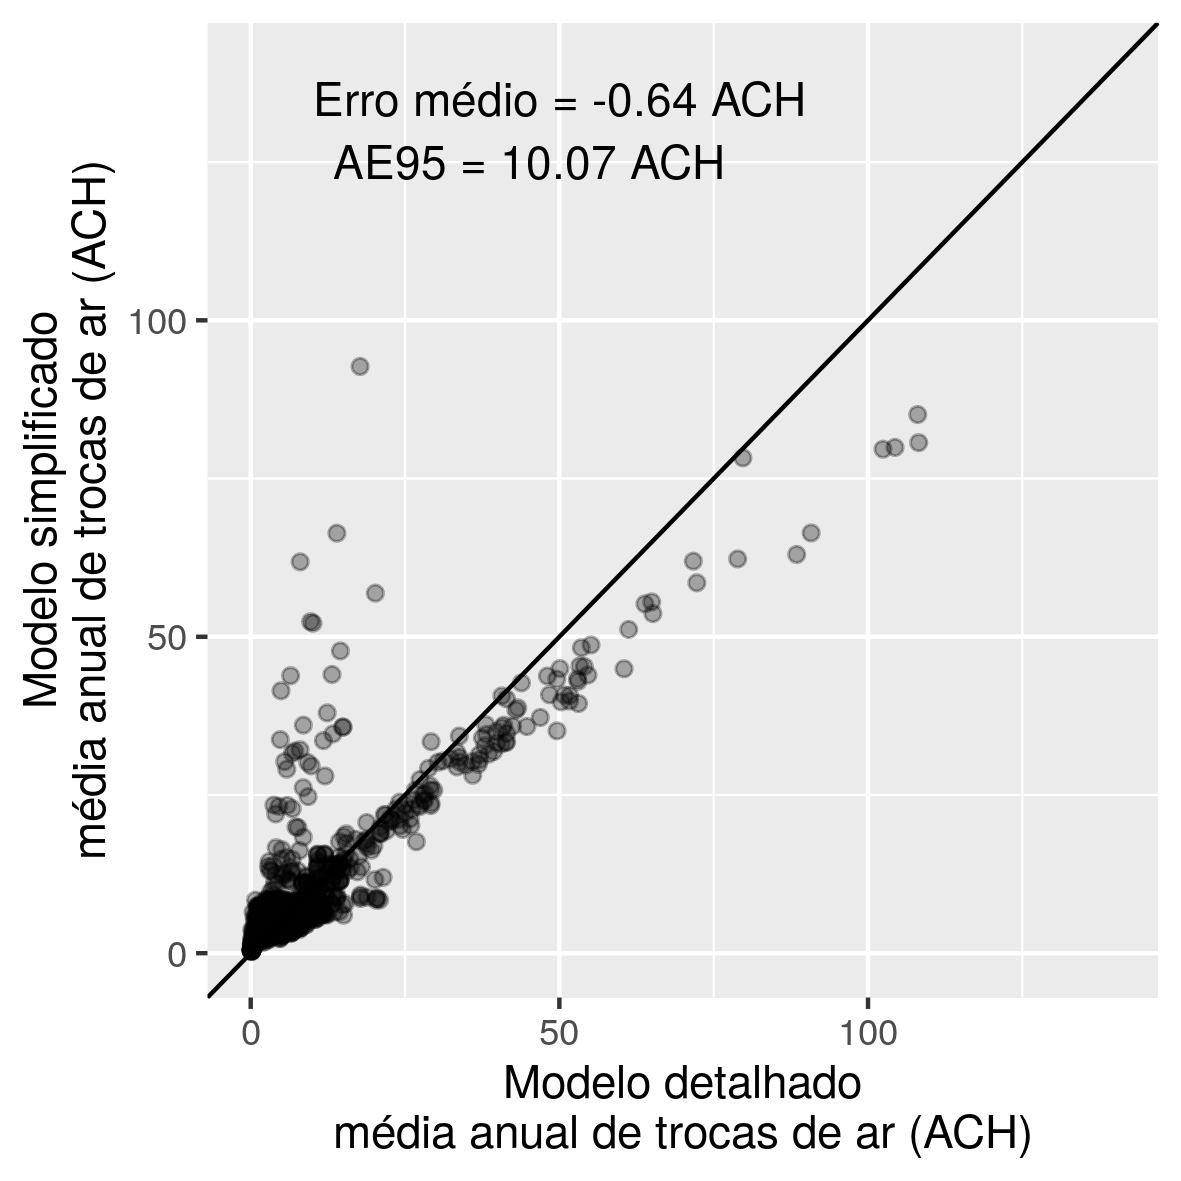
\includegraphics[width=1\linewidth]{img/cpeq_COM_10.png}
		\begin{center}
			\small{(a) comparação do \acrshort{ach}}
		\end{center}
	\end{minipage}%
	\begin{minipage}{.5\textwidth}
		\centering
		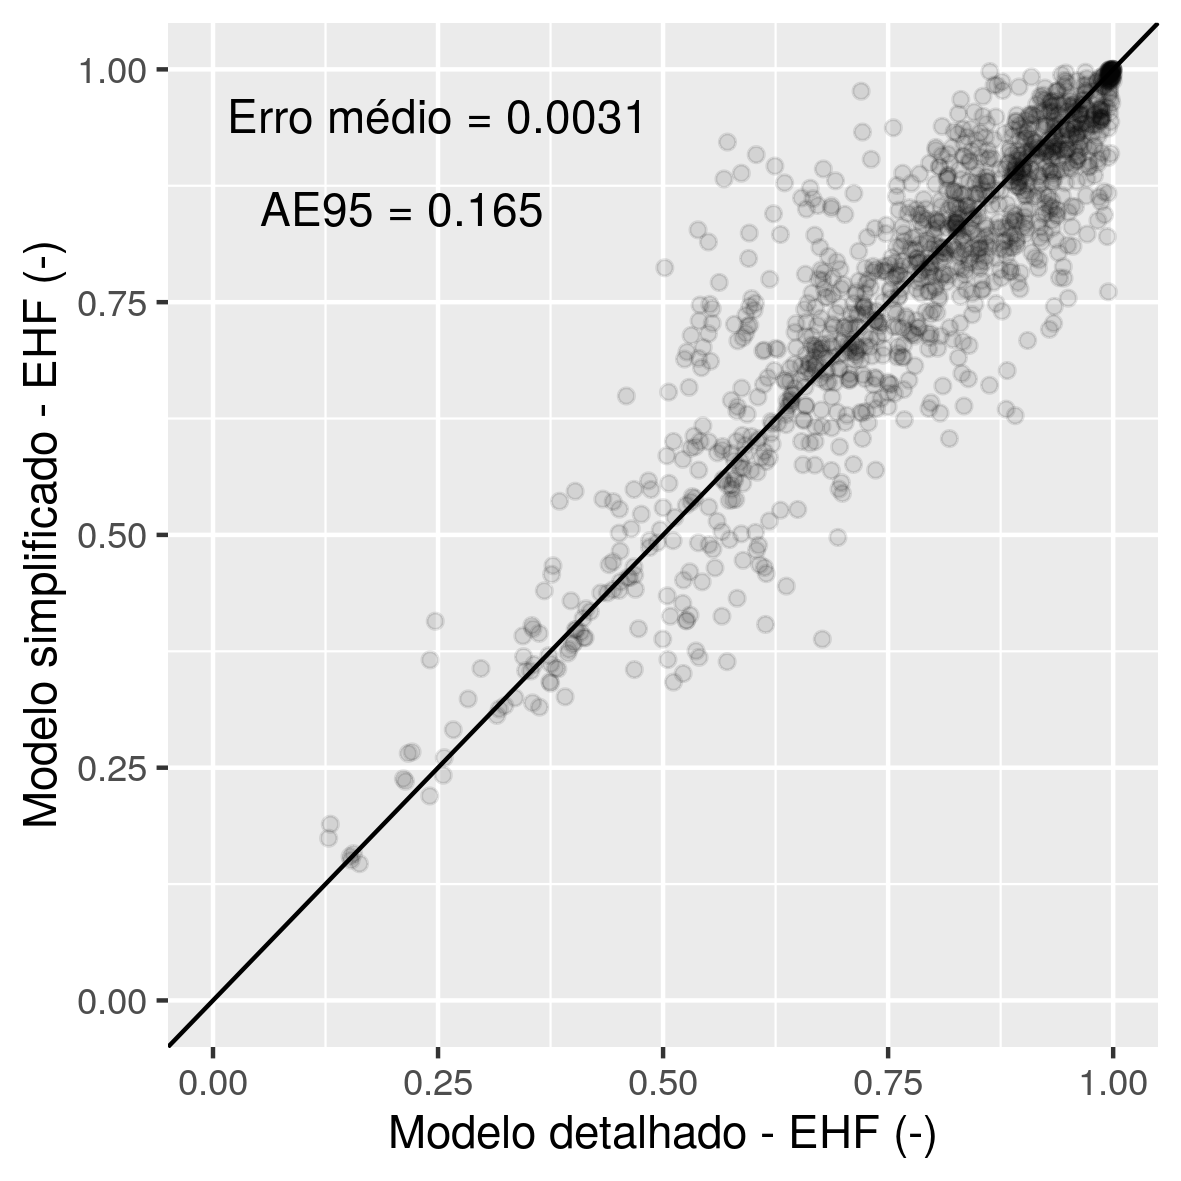
\includegraphics[width=1\linewidth]{img/cpeq_COM_10EHF.png}
		\begin{center}
			\small{(b) comparação do \acrshort{ehf}}
		\end{center}
	\end{minipage}
	\label{fig:crack01}
\end{figure}

\phantom{Linha}

Ao analisar as diferenças resultantes nas simulações simplificadas em relação às simulações detalhadas, considerou-se adequado utilizar as simplificações para a elaboração do metamodelo, e o modelo de simulação simplificada foi utilizado para as etapas posteriores: a análise de sensibilidade e o desenvolvimento do metamodelo.

\newpage

\section{Análise de sensibilidade}

As análises de sensibilidade (\acrshort{as}) foram aplicadas a partir de 155.648 simulações termoenergéticas, a partir das quais se obteve valores de \acrshort{ehf} entre 0,01 e 1,00 (Figura \ref{fig:sobol_EHF}).
A ausência de resultados de \acrshort{ehf} iguais a zero indica que, para o clima da cidade de São Paulo, o uso exclusivo de \acrshort{vn} como estratégia de resfriamento para edifícios de escritórios não é suficiente para garantir conforto térmico em todas as horas de ocupação ao longo do ano. Entretanto, a variabilidade dos resultados obtidos evidencia como o potencial de conforto térmico depende da configuração adequada dos parâmetros de projeto.
Considerando-se que, em relação às temperaturas externas, o \acrshort{ehf} para São Paulo é igual a 0,12, qualquer edificação que obtenha valores de \acrshort{ehf} inferiores a 0,12 para suas zonas térmicas já apresenta um desempenho térmico capaz de manter as temperaturas internas à edificação inferiores às externas, mesmo considerando-se as cargas internas, relacionadas a pessoas e equipamentos.

\begin{figure}[h]
	\centering
	\caption{Valores de EHF obtidos no desenvolvimento das análises de sensibilidade}
	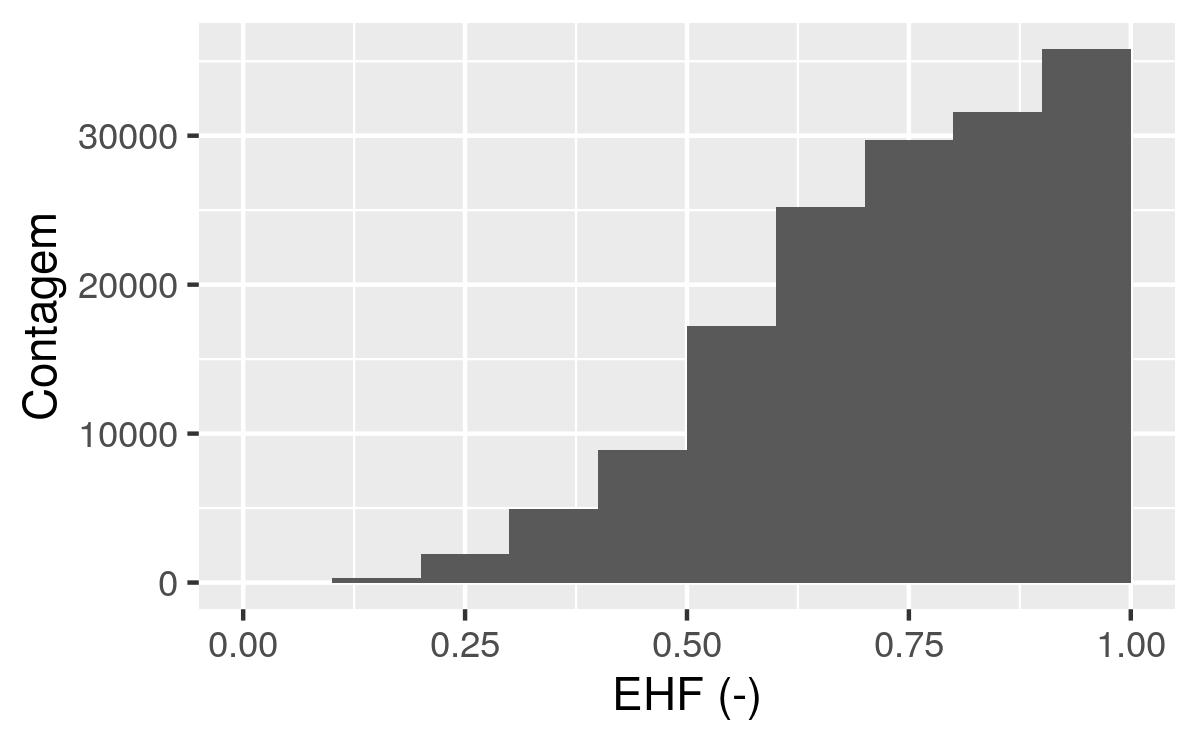
\includegraphics[width=.7\linewidth]{img/sobol_EHF.png}
	\label{fig:sobol_EHF}
	%			\begin{flushleft}
	%				Fonte: o autor.
	%			\end{flushleft}
\end{figure}

%\newpage
As Figuras \ref{fig:as_ach}, \ref{fig:as_temp} e \ref{fig:as_ehf} apresentam os resultados das análises de sensibilidade (\acrshort{as}) para efeitos de primeira ordem e efeitos totais, relacionados ao \acrshort{ehf}, às temperaturas operativas das zonas, e ao \acrshort{ehf}. Os índices apresentados são proporcionais às influências entre os dados de entrada e saída.

\begin{figure}[h]
	\centering
	\caption{Análise de sensibilidade de Sobol dos efeitos de primeira ordem e efeitos totais nas médias anuais de ACH}
	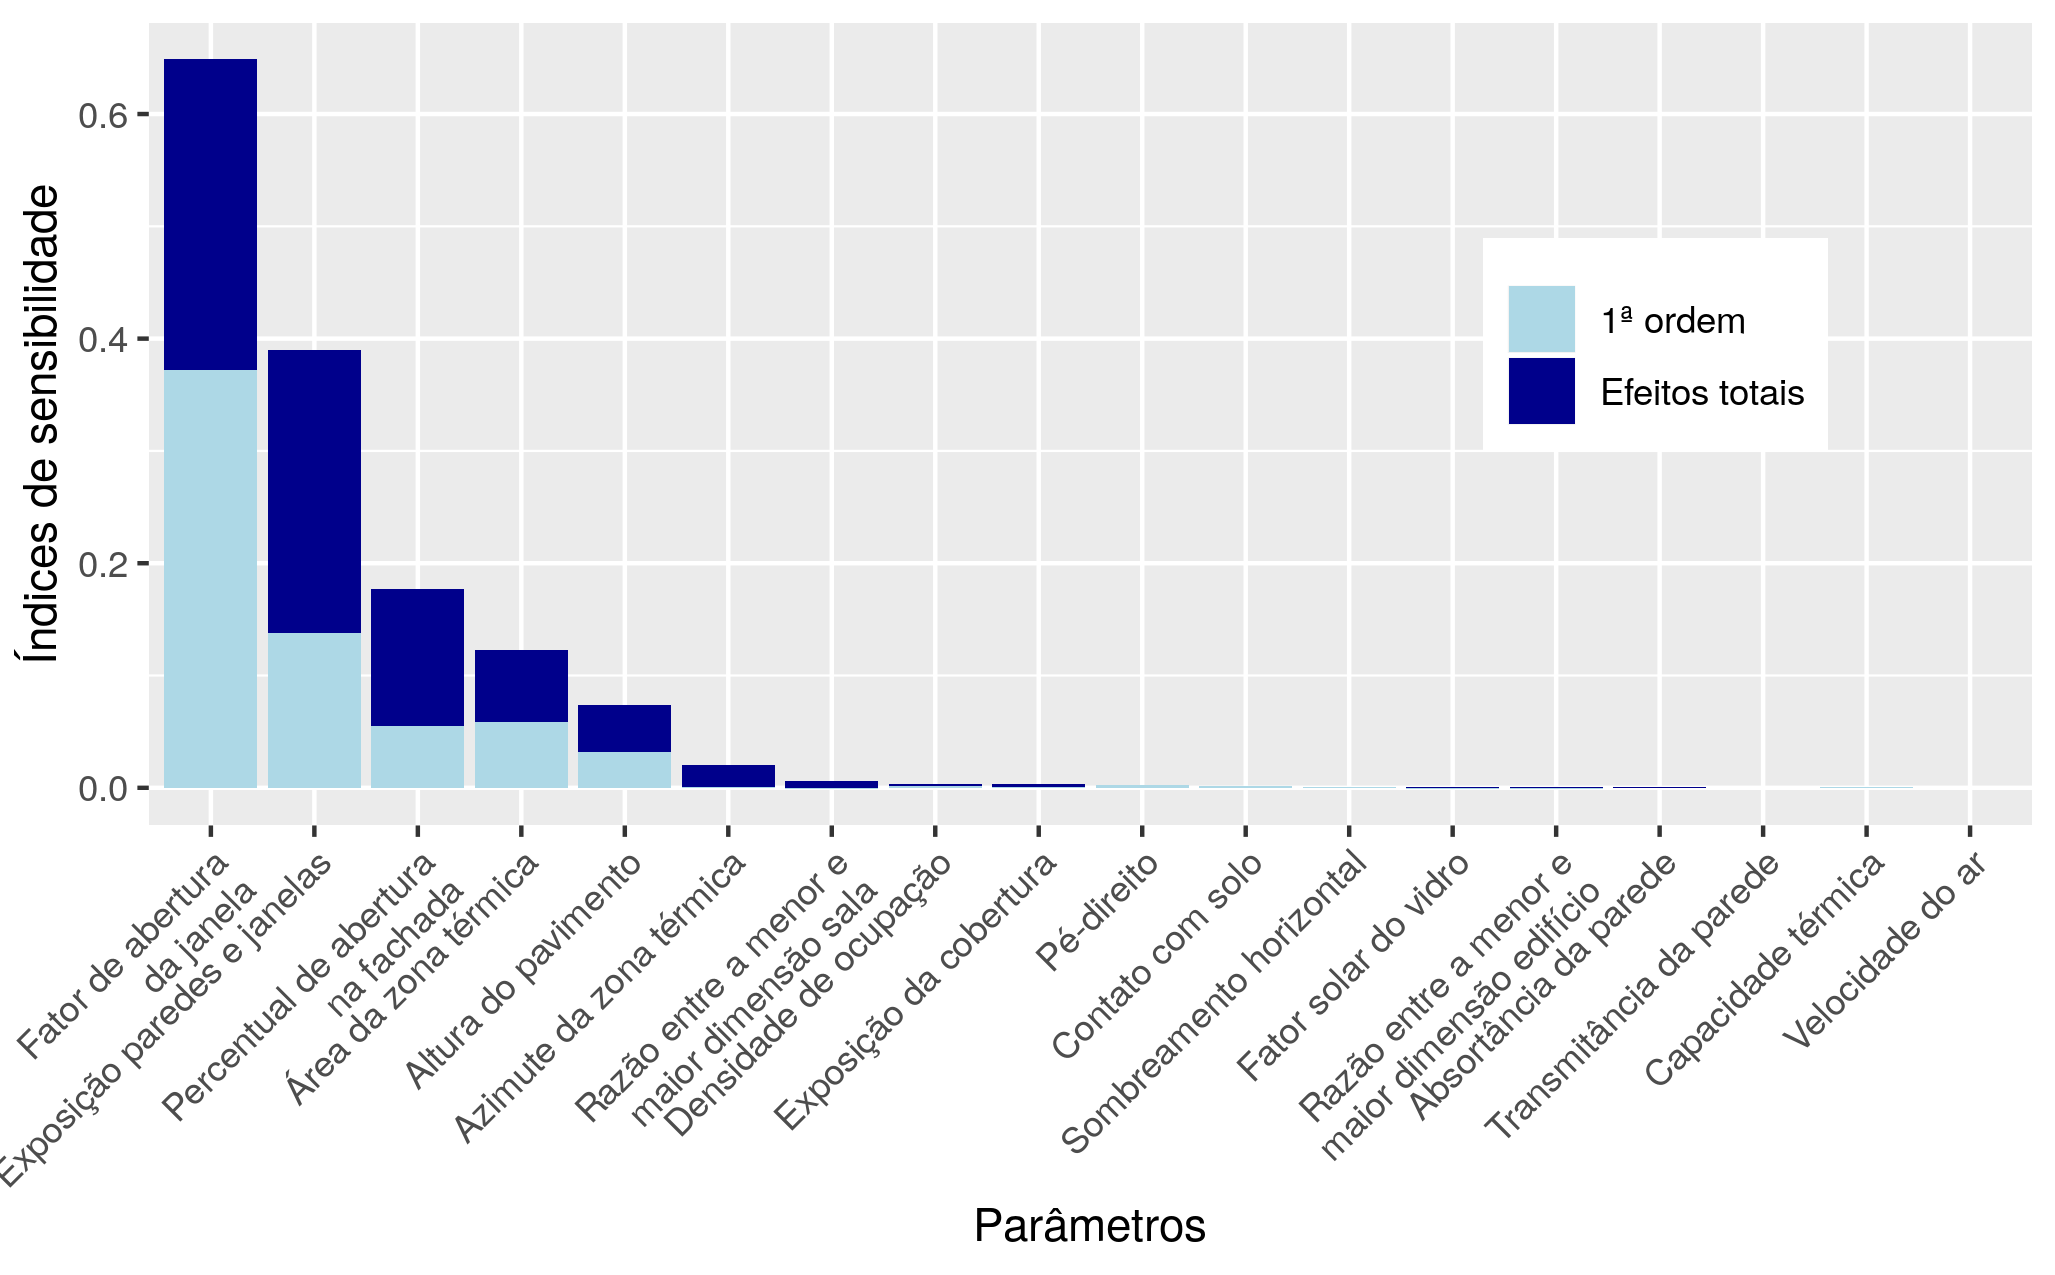
\includegraphics[width=\sasize\linewidth]{img/as_ach.png}
	\label{fig:as_ach}
	%			\begin{flushleft}
	%				Fonte: o autor.
	%			\end{flushleft}
\end{figure}

\begin{figure}[h]
\centering
\caption{Análise de sensibilidade de Sobol dos efeitos de primeira ordem e efeitos totais nas temperaturas operativas}
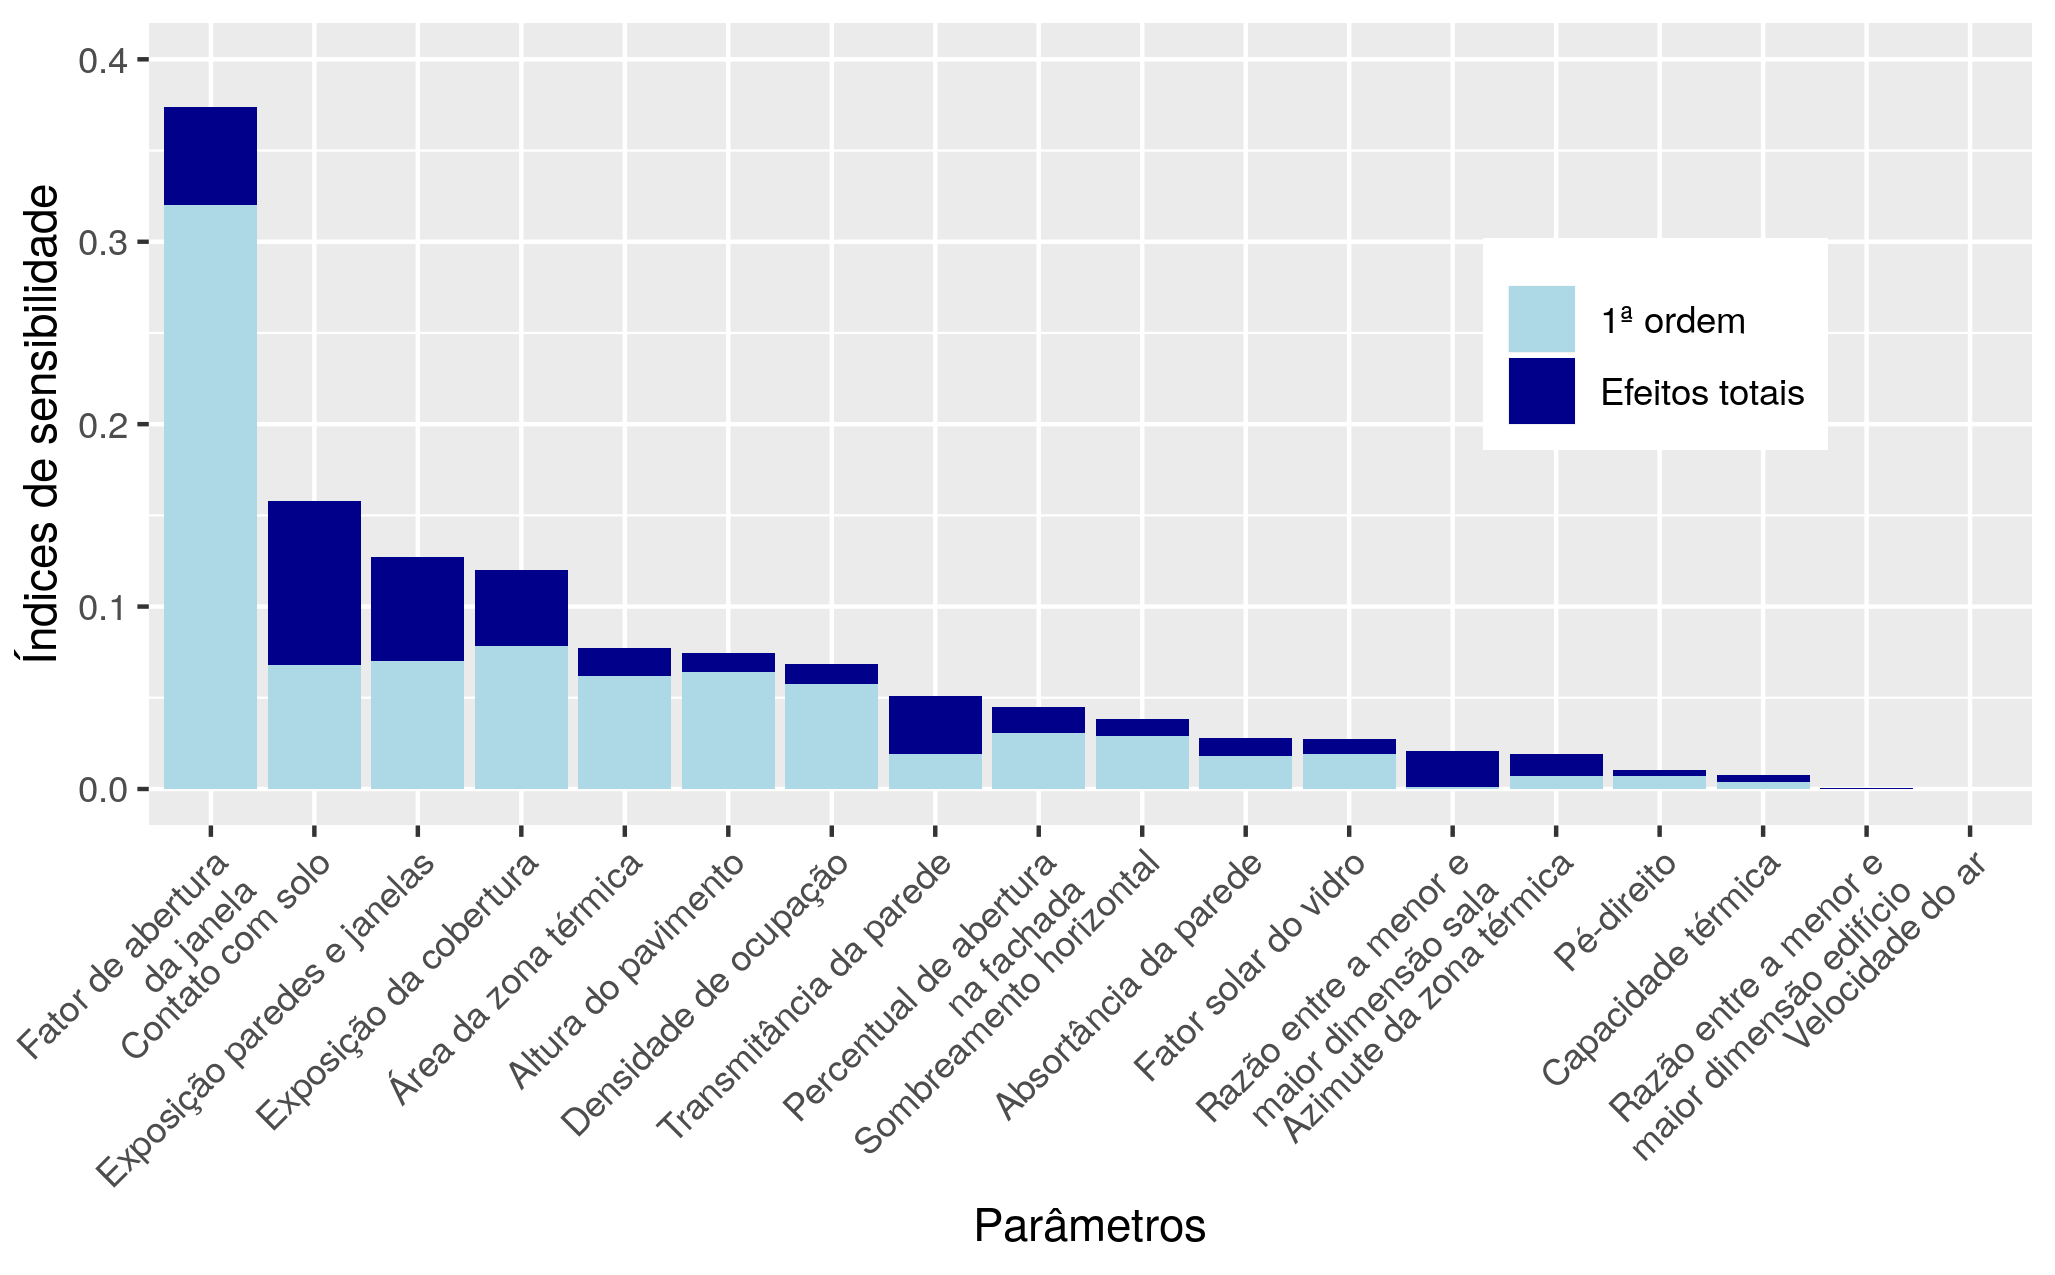
\includegraphics[width=\sasize\linewidth]{img/as_temp.png}
\label{fig:as_temp}
%			\begin{flushleft}
%				Fonte: o autor.
%			\end{flushleft}
\end{figure}

\begin{figure}[h]
\centering
\caption{Análise de sensibilidade de Sobol dos efeitos de primeira ordem e efeitos totais no EHF}
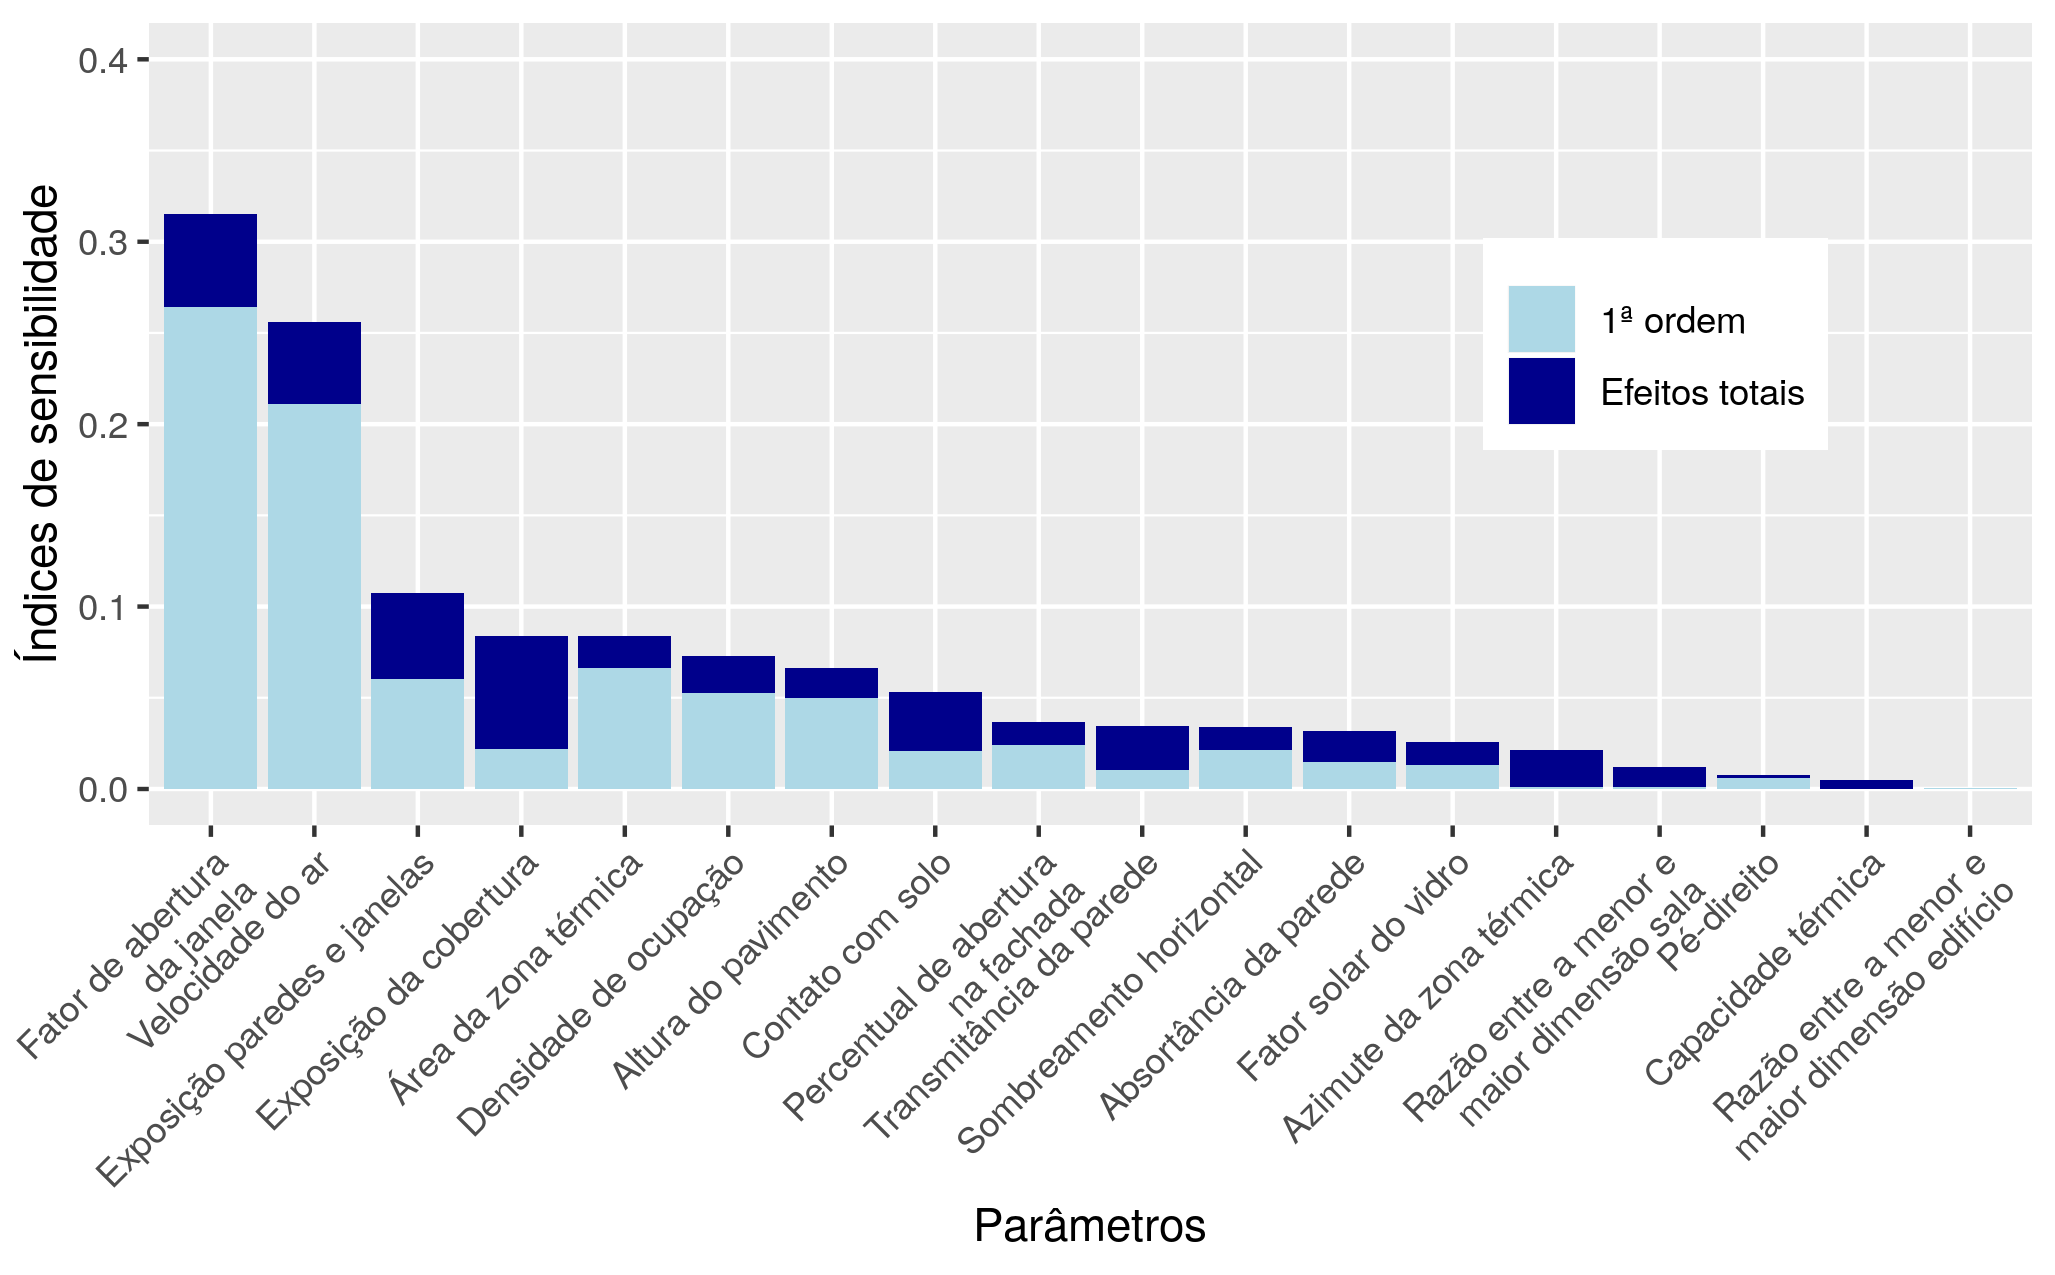
\includegraphics[width=\sasize\linewidth]{img/as_ehf.png}
\label{fig:as_ehf}
%			\begin{flushleft}
%				Fonte: o autor.
%			\end{flushleft}
\end{figure}

Os parâmetros mais influentes no \acrshort{ach}, como esperado, são aqueles relacionados às aberturas da zona. 
O primeiro parâmetro de maior influência é o fator de abertura das janelas, seguido do parâmetro relacionado à exposição das paredes e à presença de \acrshort{vn} cruzada ou unilateral. 
A área da zona  térmica tem influência significativa, pois o cálculo das trocas de ar leva em conta o volume de ar na zona, que é diretamente relacionado à sua área. 
A altura do pavimento é determinante nos resultados do \acrshort{ach}, pois a velocidade do vento no EnergyPlus é calculada em função da altura da zona.
A orientação da zona (azimute) não tem uma influência significativa de primeira ordem. No entanto, percebe-se uma influência mais significativa considerando-se os efeitos totais. 
O azimute é determinante para a definição dos coeficientes de pressão sobre as fachadas da edificação. Por isso, a influência deste parâmetro nos resultados das simulações depende de outros parâmetros, relacionados ao posicionamento e às áreas das aberturas na zona.
A velocidade do ar não influencia os resultados relacionados ao \acrshort{ach}, pois é considerada somente após o término das simulações, ao se calcular o \acrshort{ach}.
A \acrshort{as} apresentou interações de segunda ordem significativas entre o fator de abertura das janelas e a presença de \acrshort{vn} cruzada ou unilateral, com um índice de sensibilidade igual a 0,121.
Contudo, o parâmetro com maiores interações de segunda ordem relacionados ao \acrshort{ach} foi o \acrshort{paf}, com a soma dos índices de segunda ordem igual a 0,300.

As análises relacionadas à temperatura operativa e ao \acrshort{ehf} indicam relevância dos parâmetros relacionados à \acrshort{vn}. Para ambas as análises, o parâmetro mais influente foi o fator de abertura da janela, enquanto o parâmetro relacionado à exposição das paredes e à presença de \acrshort{vn} cruzada ou unilateral foi o terceiro mais influente. 
O contato com o solo apresentou-se como o segundo parâmetro mais influente nas médias anuais de temperatura operativa, considerando-se os esfeitos totais. No entanto, a influência deste parâmetro não é tão significativa no \acrshort{ehf}. Isso indica que a influência do contato com o solo nas temperaturas operativas das zonas é mais significativa em faixas de temperatura que não interferem no cálculo do \acrshort{ehf}, ou seja, consideravelmente acima ou abaixo dos limites superiores de aceitabilidade estabelecidos pelo método de conforto adaptativo.
Observa-se que os efeitos totais entre o segundo (contato com o solo) e o quarto (exposição da cobertura) índice de sensibilidade com valores mais altos na \acrshort{as} relacionada à média anual da temperatura operativa são expressivos.
A transmitância das paredes, o azimute, e a razão entre a largura e o comprimento da sala também apresentam efeitos totais relevantes, apesar dos baixos índices de sensibilidade para primeira ordem. Isso indica que há interações significativas entre esses parâmetros e os demais.

O movimento do ar apresenta-se como o segundo parâmetro mais influente nos resultados de \acrshort{ehf}, o que indica um grande potencial de uso de ventiladores na busca por conforto térmico nos ambientes. 
A área da zona e a densidade de ocupação apresentaram-se mais influentes nos resultados de \acrshort{ehf}, comparando-se aos resultados relacionados às médias anuais de temperatura operativa.
O azimute, apesar de seu índice de sensibilidade baixo para a análise de primeira ordem, apresentou índices de segunda ordem expressivos. As interações de segunda ordem ocorrem relacionadas a parâmetros referentes à \acrshort{vn} e a parâmetros referentes à radiação solar. A soma dos índices de segunda ordem do azimute em relação ao \acrshort{ehf} foi igual a 0,177.  %, como sombreamento e absortância

A complexidade dos fenômenos representados junto às interações entre as diferentes variáveis exige um grande número de casos para reduzir incertezas, pois o método de \acrshort{as} utiliza uma base amostral. Por isso, existe uma incerteza associada aos índices de sensibilidade obtidos nas \acrshort{as} conduzidas, e a soma dos valores dos índices ultrapassa o valor 1. Entretanto, a aplicação da análise de sensibilidade global ofereceu resultados relevantes para o trabalho, com índices de sensibilidade condizentes aos comportamentos físicos representados pelas simulações. 

Baseando-se nos resultados das \acrshort{as}, alguns dos parâmetros não foram considerados para o desenvolvimento do metamodelo. Desconsiderar parâmetros com índices de sensibilidade significativamente baixos possibilita o desenvolvimento de um metamodelo mais simples, com menos dados de entrada e maior precisão nos resultados. Os parâmetros desconsiderados tiveram seus valores fixados, de acordo com a Tabela \ref{table:param_fixed}. O valor do pé-direito foi determinado considerando-se o valor encontrado com mais frequência na base de dados analisada. A capacidade térmica da parede foi estabelecida de acordo com o valor de uma parede de bloco cerâmico de dimensões 14x19x29 cm, e argamassa de 2,5 cm, resultando em um valor de 161 kJ/m$^2$K. No entanto, como as simulações foram desenvolvidos com o modelo de parede equivalente, considerou-se apenas metade do valor da capacidade térmica. Os parâmetros relacionados às proporções entre largura e profundidade das salas e edifícios foram determinados com valor igual a 1. 

\begin{table}[h]		
	\centering
	\caption{Parâmetros com valores constantes}
	\label{table:param_fixed}
	\begin{tabular}{|l |c |}
		\hline
		\textbf{Parâmetro} & Valor fixo \\
		\hline
		Razão entre a menor e maior dimensão do edifício ($-$) & 1 \\
		\hline
		Razão entre a menor e maior dimensão da sala ($-$) & 1 \\
		\hline
		Pé-direito ($m$) & 2,5 \\
		\hline
		Capacidade térmica ($kJ/m^2K$) & 80 \\
		\hline
		%			Fator solar do vidro ($-$) & 0,87 \\
		%			\hline
	\end{tabular}
\end{table}

\newpage

\section{Desenvolvimento do metamodelo}

O metamodelo final foi definido com 14 parâmetros:
\begin{itemize}
	\item Fator de abertura das janelas;
	\item Velocidade do ar;
	\item Condição de exposição das paredes e janelas;
	\item Área da sala;
	\item Densidade de ocupação;
	\item Altura do pavimento;
	\item Exposição da cobertura;
	\item Sombreamento horizontal;
	\item Contato com o solo;
	\item Transmitância das paredes;
	\item Absortância das paredes;
	\item Fator solar do vidro;
	\item Azimute da sala;
	\item \Acrlong{paf}.
\end{itemize}

As 100.000 simulações termoenergéticas foram desenvolvidas para o treinamento da rede neural artificial (\acrshort{ann}) a partir de combinações entre os parâmetros definidos.
Os parâmetros variaram na mesma faixa de valores estabelecida na Seção \ref{section:parametrosdeentrada}. O ângulo do azimute da sala é determinado considerando-se o eixo entre a parede voltada para a circulação e a parede oposta à circulação.
O contato com o solo e a exposição da cobertura foram definidas como variáveis binárias, com o valor zero correspondendo à superfície adiabática, e 1 correspondendo à exposição.
O parâmetro que representa a condição de exposição das paredes e janelas não foi representado com valores numéricos, e sim como uma variável de fatores, com cinco opções de exposição. Além das três opções apresentadas na Figura \ref{fig:exp_sz}, considerou-se também as exposições espelhadas. 	
Os demais parâmetros foram normalizados com valores entre -1 e 1.

\begin{figure}[h]
	\centering
	\caption{Condição de exposição das paredes e janelas}
	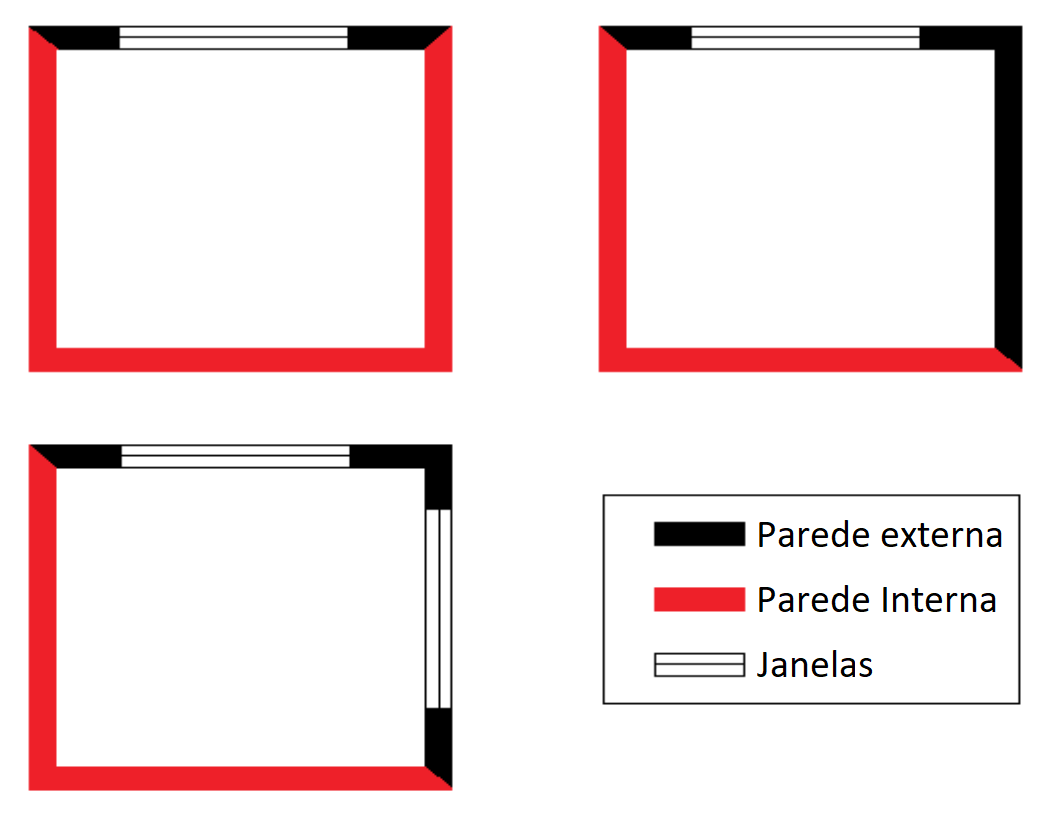
\includegraphics[width=.5\linewidth]{img/wallexposition2.png}
	\label{fig:exp_sz}
	%			\begin{flushleft}
	%				Fonte: o autor.
	%			\end{flushleft}
\end{figure}

O modelo de \acrshort{ann} final foi definido com duas camadas, umas de 50 nós, e a outra com 20. 
O algorítimo de otimização que obteve o melhor desempenho foi o \textit{Adagrad's Optimizer}, disponibilizado pela biblioteca \textit{TensorFlow} \cite{tensorflow2015}, com uma taxa de aprendizagem igual a 0,05. O treinamento foi interrompido após 150.000 iterações. Neste momento, os erros de obtidos para as estimativas da amostra de validação pararam de baixar, e continuar o processo poderia causar o um sobreajuste do metamodelo em relação à amostra de treinamento.

A Figura \ref{fig:ann_validation} apresenta um gráfico de pontos comparando os resultados de \acrshort{ehf} obtidos para as simulações e para as estimativas da \acrshort{ann}, a partir da base de dados desenvolvida para a validação do metamodelo. A base de dados para a validação (Figura \ref{fig:ann_validation}a) teve apenas os parâmetros incluídos no treinamento da \acrshort{ann} variados. 
O erro absoluto médio do \acrshort{ehf} para os casos de validação foi 0,0091, com o \acrshort{ae95} igual a 0,0244.
Para essa amostra, a \acrshort{ann} não superestimou, nem subestimou significativamente os resultados, revelando uma diferença média entre os resultados preditos e simulados igual a 0,0003.

\begin{figure}[h]
	\caption{Comparação entre os resultados de EHF estimados pelo metamodelo e simulados pelo Energyplus}
	\begin{minipage}{.5\textwidth}
		\centering
		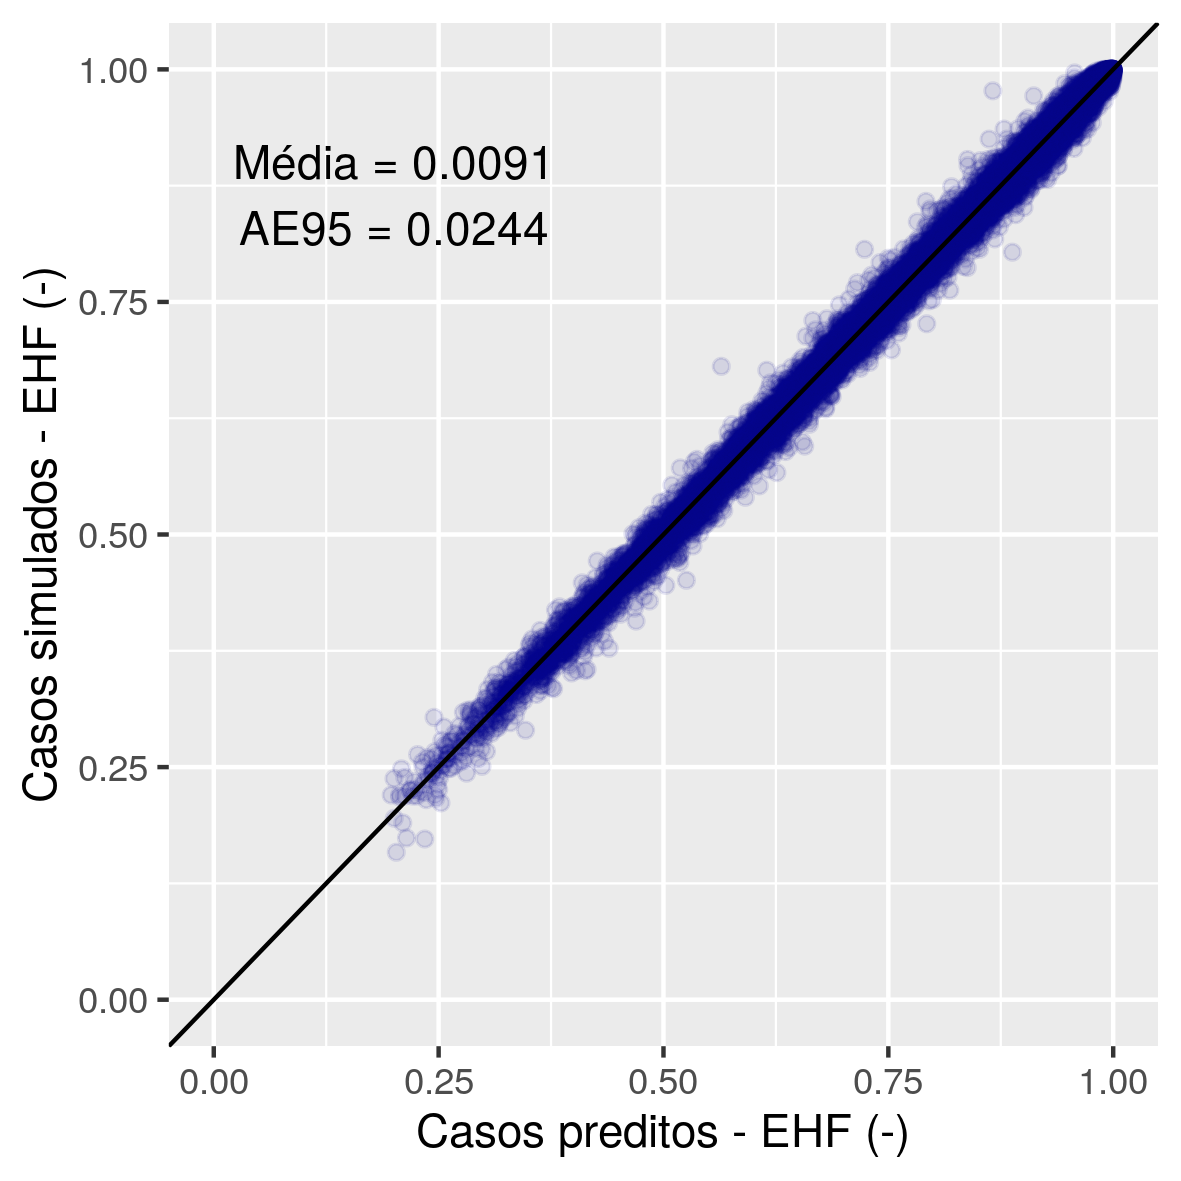
\includegraphics[width=1\linewidth]{img/ann_validation.png}
		\begin{center}
			\small{(a) Amostra de validação}
		\end{center}
	\end{minipage}%
	\begin{minipage}{.5\textwidth}
		\centering
		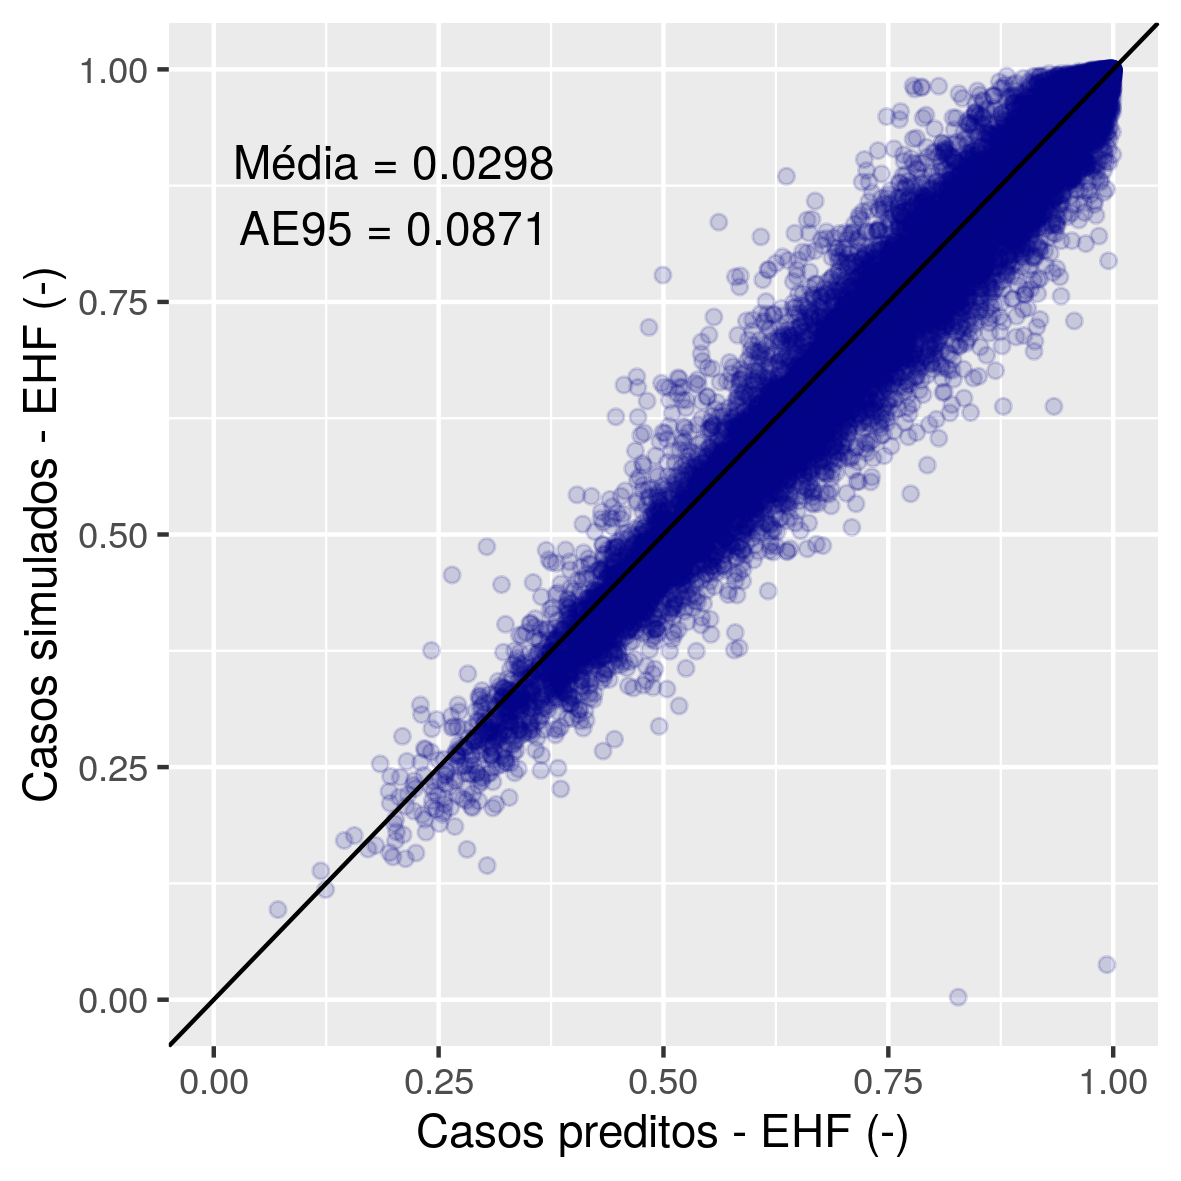
\includegraphics[width=1\linewidth]{img/ann_test.png}
		\begin{center}
			\small{(b) Amostra de teste}
		\end{center}
	\end{minipage}
	\label{fig:ann_validation}
\end{figure}

%\begin{figure}[H]
%	\centering
%	\caption{Condição de exposição das paredes e janelas}
%	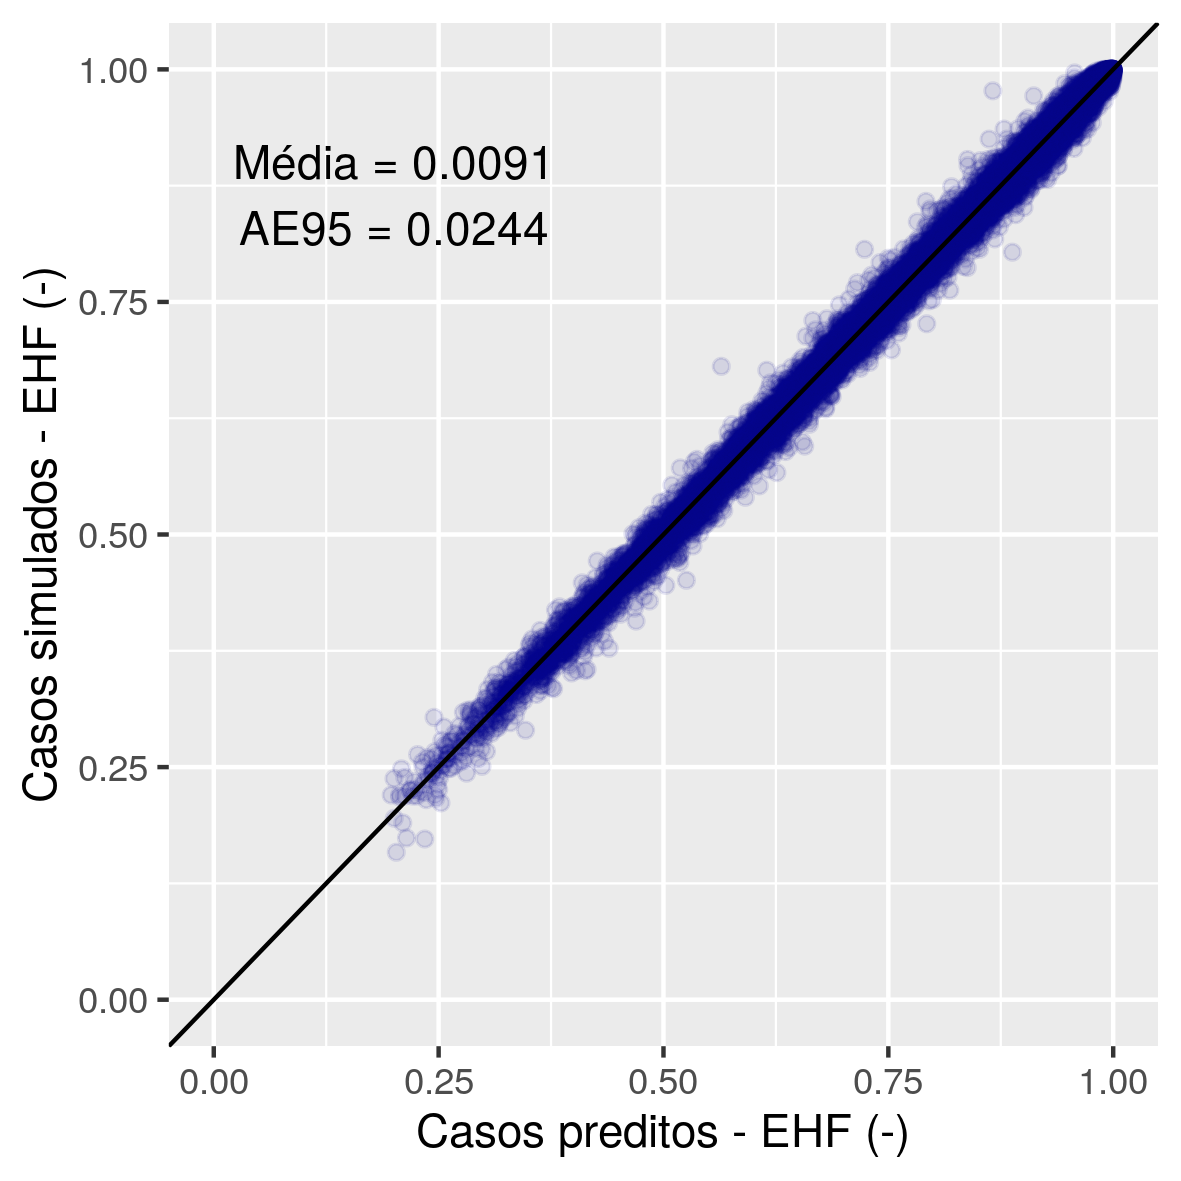
\includegraphics[width=.5\linewidth]{img/ann_validation.png}
%	\label{fig:ann_validation}
%\end{figure}

Para verificar as incertezas geradas nos resultados quando os parâmetros não incluídos como dados de entrada da \acrshort{ann} variam, outra amostra foi gerada para teste, com 20.000 casos.
A Figura \ref{fig:ann_validation}b apresenta o gráfico de pontos comparando os resultados de \acrshort{ehf} obtidos para as simulações e para as estimativas da \acrshort{ann}, a partir da base de dados gerada para verificar o impacto das incertezas no resultados. O erro absoluto médio do \acrshort{ehf} para os casos de validação foi 0,0298, com o \acrshort{ae95} igual a 0,0871.
No gráfico, é possível observar que os resultados para amostra de teste apresentam um enviesamento nas estimavas do \acrshort{ehf}, que retornam valores mais altos do que os obtidos pelas simulações. Essa diferença se faz mais expressiva em faixas de valores mais baixas de \acrshort{ehf}. Para os casos simulados com resultados de \acrshort{ehf} inferiores a 0,50, as estimativas de \acrshort{ehf} obtidas pela \acrshort{ann} são em média 0,0315 mais altas.

Os resultados obtidos pelo metamodelo desenvolvido apontam que a \acrshort{ann} é capaz de estimar adequadamente o conforto térmico em relação aos resultados simulados pelo programa EnergyPlus. 
Apesar das diferenças observadas entre os resultados preditos e simulados, os erros não são expressivos a ponto de impedir o uso da ferramenta.
Em situações em que há a necessidade de respostas rápidas, sem a possibilidade de utilizar-se programas de simulação computacional, como o EnergyPlus, a \acrshort{ann} desenvolvida pode ser aplicada, de maneira simples, para oferecer respostas relacionadas ao desempenho térmico de edifícios de escritório.

%\begin{figure}[H]
%	\centering
%	\caption{Condição de exposição das paredes e janelas}
%	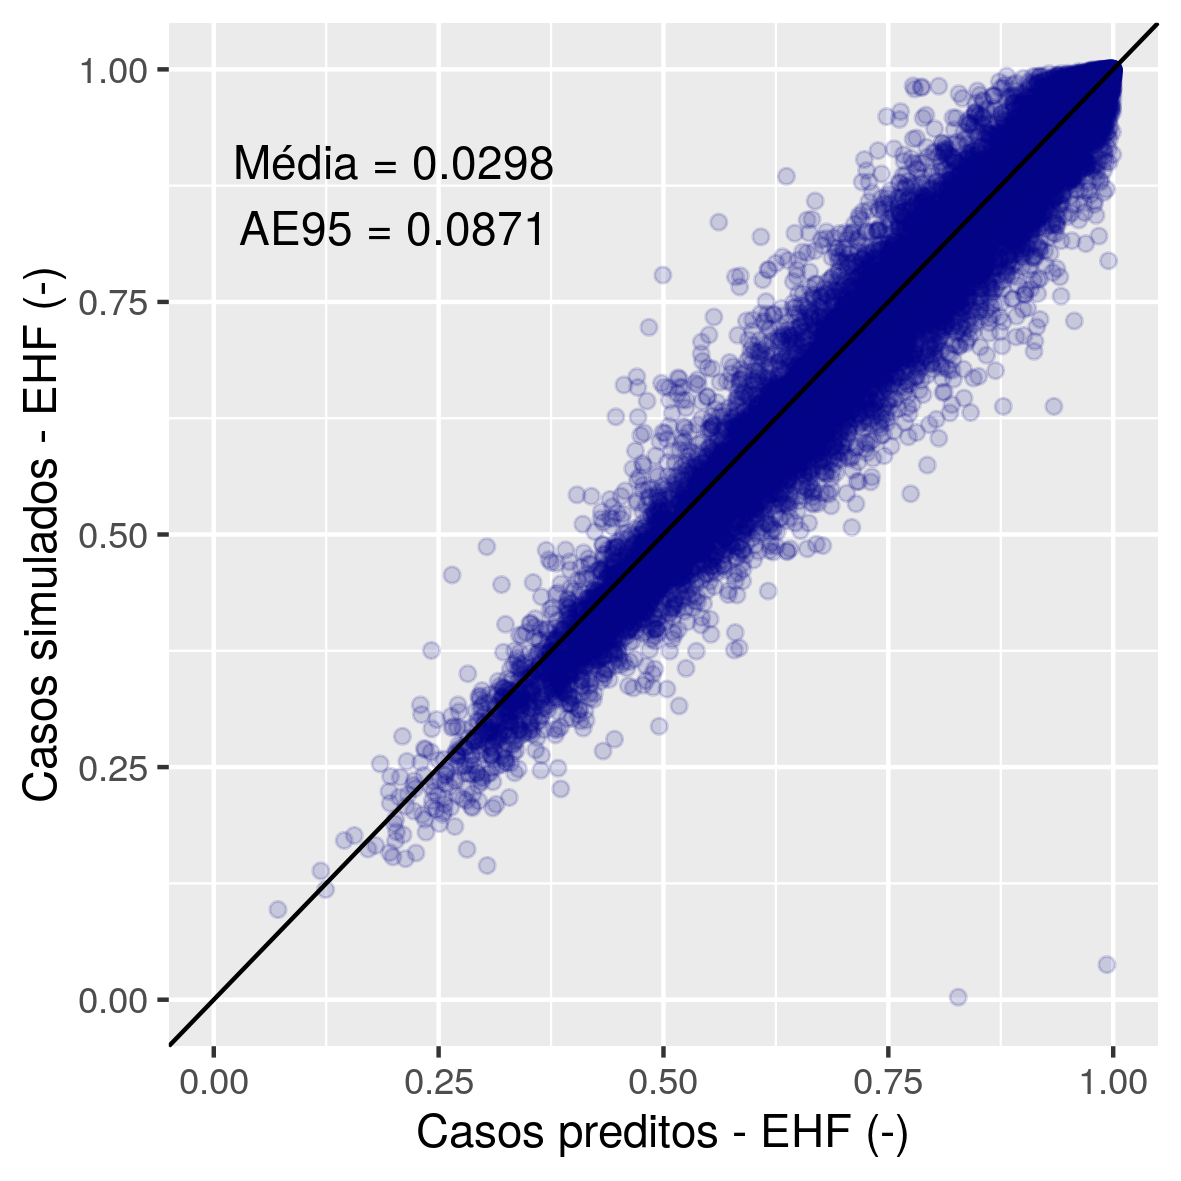
\includegraphics[width=.5\linewidth]{img/ann_test.png}
%	\label{fig:ann_sobol}
%\end{figure}